\documentclass[12pt]{article}
\usepackage{graphicx}
\textwidth 17cm
\oddsidemargin -0.54cm  %2cm Rand links
\topmargin 0.46cm %3cm Rand oben
\headheight 0cm % no header
\headsep 0cm
\textheight 22cm
\parskip 6pt
\parindent 0pt

\newcommand{\biburl}[1]{{\small{\tt #1}}}

\newenvironment{mylist}
  {\begin{list}{$\bullet$}{\parsep 0pt}}
  {\end{list}}
\newenvironment{mysublist}
  {\begin{list}{$-$}{\parsep 0pt \topsep 0pt \leftmargin 2cm}}
  {\end{list}}
\newcommand{\degree}{\mbox{$^{\circ}$}}
\newcommand{\see}{\mbox{$\rightarrow$}}
\newcommand\beq{\begin{equation}}
\newcommand\eeq{\end{equation}}
\newcommand{\uvec}[1]{\mbox{$\hat{\vec{#1}}$}}
\newcommand{\cvec}[1]{\mbox{$\underline{\vec{#1}}$}}
\newcommand{\csca}[1]{\mbox{$\underline{#1}$}}
\newcommand{\Tr}{{\rm Tr}}
\newcommand{\sign}{{\rm sign}}
\newcommand\pt{\partial}
\newcommand{\tilvec}[1]{\vec{\tilde{#1}}}



\newcommand\todo[1]{$\Longrightarrow$ {\em #1} }
%\newcommand\bug[1]{$\Longrightarrow$ {\em #1} }
\newcommand\code[1]{{\tt [#1]}}

\newcommand\opamodule[3]{{\bf \tt #1} #2\\  \rule[3pt]{\textwidth}{0.2pt} \\ {\scriptsize uses \tt  #3}\\[1ex]}
\newcommand\opamoduleN[2]{{\bf \tt #1} #2\\  \rule[3pt]{\textwidth}{0.2pt} \\}



\begin{document}\noindent

\parbox[t]{0.7\hsize}{
  {\Huge\bf inside OPA} version {\bf 4.061}\\
  Andreas Streun, PSI, \today
} \hfill  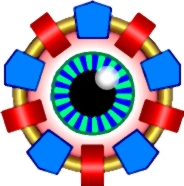
\includegraphics{opalogo_small.jpg}
\rule{\hsize}{1pt}
\section{Introduction}

This note documents the beam dynamics algorithms used in and partially developed for OPA during the past decades. It may help OPA users to understand the meaning of the results and the limitations of the models used.

For programmers who like to further develop or renew OPA, or only want to reuse some piece of the code or an algorithm in other projects, we refer to the relevant units and procedures or functions by \code{Unit> Procedure}-- occasionally some more comment may be found there. A brief description of the OPA units is given in Appendix \ref{appunits}.

The remark \todo{to do\dots} gives suggestions were things could be completed or improved in future.

This note is subject to continuous changes as OPA development proceeds further.

\section{Beam optics}

OPA uses the most simple accelerator model: the lattice is a concatenation of elements, which are either long ($L\geq 0$) and linear and described by a symplectic transfer matrix, or thin ($L=0$) and non-linear and described by a single kick map. Long non-linear elements are modeled as a series of drifts and kicks (which corresponds to a basic second order symplectic integrator).

OPA is a code for transverse beam dynamics and does not include longitudinal dynamics (i.e. acceleration). An offset from design momentum $u=\Delta p/p_o$ is considered as constant (adiabatic approximation). The transfer matrices are of size $5\times 5$ where the fifth row is just $(0,0,0,0,1)$. Thus they propagate the particle vector $(x,x',y,y',u)^T$ without changing $u$.

OPA uses the highly relativistic, paraxial and large-ring approximations as detailed in appendix \ref{ssechamapp}. It's main area of application are high energy electron storage rings.\\

Up to version~3 OPA was restricted to flat lattices (only vertical bends, no skew elements), where horizontal and vertical motion are decoupled and all transfer matrices are block-diagonal. In version~4 the Sagan-Rubin representation \cite{SAGAN} of the Edward-Teng formalism \cite{EDTENG} was implemented as a major upgrade in order to include transverse coupling: it introduces the ``normal-mode transformation'', where the two transverse planes are decoupled again, but they do not correspond anymore to the physical planes $x$ and $y$, and therefore are denoted $a$ and $b$.

Linear beam optics at any location in the accelerator in general is fully described by the orbit, which is a 4-vector, accompanied by the scaler momentum offset $u$, the Twiss parameters of the two transverse planes (beta and alpha-functions), and the dispersion 4-vector $\vec{D}=(D_x,D_x',Dy,D_y')^T$. In coupled lattices, in addition the $2\times 2$ coupling matrix $C$ is required; then the Twiss parameters correspond to the ``normal modes''.


\subsection{The Periodic solution}
Beam parameters along the lattice are calculated by propagating initial parameters.
In a circular lattice (storage ring), the periodic solutions have to be calculated beforehand to generate the initial parameters.

The closed orbit is the fixpoint of the one-turn map including also kicks from non-linear elements. It is iteratively found by application of the standard Newton-Raphson root finding method using the {\em local} transfer matrix (i.e. the one turn matrix including gradient down feeds from non-linear multipoles) as the Jacobian, i.e. as the gradient for the root finder \code{OpticPlot> ClosedOrbit}.

When the orbit is found, the local transfer matrix is used to find the periodic dispersion and the (normal mode) Twiss parameters as described in \cite{SAGAN}:
The $5\times 5$ one-turn matrix is composed from a the $4\times 4$ transverse focusing matrix $R$ and the 4-vector of dispersion production $\vec{Z}$, with $2\times 2$ sub-matrices non-coupling $M,N$ and coupling $m,n$ and horizontal and vertical 2-vectors of dispersion production $\vec{V}, \vec{w}$:
\beq
R = \left(\begin{array}{cc} N & m \\ n & N \end{array}\right)\qquad \vec{Z}=\left(\begin{array}{c}\vec{V} \\ \vec{w}\end{array}\right)
\eeq
A normal mode decomposition of $R$ may be found~\
\begin{equation}\label{eq:edteng}
R= T^{-1} {\cal G}^{-1} {\cal O} {\cal G} T
\end{equation}
where $\cal O$ is the matrix containing the eigen-tunes
\begin{equation}\label{eq:eigentune}
{\cal O} =\left(\begin{array}{cc} {O}_a & 0 \\ 0 & {O}_b\end{array}\right)
\quad\mathrm{and}\quad
{O}_{a,b}=\left(\begin{array}{rc} \cos\mu_{a,b} & \sin\mu_{a,b} \\ -\sin\mu_{a,b} & \cos\mu_{a,b}\end{array}\right)
\end{equation}
and ${\cal G}$ is the matrix that contains the local normal-mode beta functions. It is given by
\begin{equation}\label{eq:calA}
{\cal G} = \left(\begin{array}{cc} {G}_a & 0 \\ 0 & {G}_b\end{array}\right)
\quad\mathrm{and}\quad
{G}_{a,b} =
\left(\begin{array}{cc} \frac{1}{\sqrt{\beta_{a,b}}} & 0 \\ \frac{\alpha_{a,b}}{\sqrt{\beta_{a,b}}} & \sqrt{\beta_{a,b}}
\end{array}\right)
\end{equation}
where the indices $a$ and $b$ label the two eigen modes.
It is related to the normalized and periodic sigma matrix
\beq\label{eq:signorm}
S_{a,b} =  G_{a,b}^{-1}{G}_{a,b}^{-T} =
\left( \begin{array}{cc} \beta_{a,b} & -\alpha_{a,b} \\
-\alpha_{a,b} & \gamma_{a,b} \end{array} \right)\quad\mbox{with}\quad \gamma_{a,b}=\frac{1+\alpha^2_{a,b}}{\beta_{a,b}}.
\eeq
The coupling matrix $T$ and its inverse $T^{-1}$ are given by~\cite{SAGAN}
\beq\label{eq:tmatrix}
T=\left( \begin{array}{cc} gI & -C \\ C^+ & gI \end{array} \right)
\qquad \mathrm{and}\qquad
T^{-1}=\left( \begin{array}{cc} gI & C \\ -C^+ & gI \end{array} \right) ,
\eeq
with the $2\times 2$ identity matrix $I$ and the $2\times 2$ coupling matrix $C$.
Its symplectic conjugate $C^{+}$ and the scalar $g$ are given by
\beq
C^+=C^{-1}\det C ,\quad \mbox{\rm and}\quad  g^2=1-\det C.
\eeq
Explicit calculations are described in \cite{SAGAN}. For the coupling terms they derived
\beq
g=\sqrt{\frac{1}{2}\pm\frac{1}{2}\frac{|\Tr (M-N)|}{h}}\qquad
C=\mp  \frac{\sign (\Tr (M-N))}{g\,h}(m+n^+)
\eeq
\beq
\mbox{\rm with}\quad h=\sqrt{(\Tr(M-N))^2+4 \det (m+n^+)}.
\eeq
Existence of a periodic solution corresponds to a real value of $h$. The normal mode transformation is not always unique, and a second solution exists for $\det (m+n^+)>0$ as indicated by the lower sign in the equations. Usually the upper sign is valid in weakly coupled lattices. Knowing the coupling terms, the normal-mode beta functions are calculated as\footnote{note, that the first version of \cite{SAGAN} had an erratum here}:
\begin{eqnarray}
 A &= &  {G}_a^{-1} {O}_a {G}_a = \left(\begin{array}{cc} \cos\mu_a +\alpha_a \sin \mu_a & \beta_a \sin\mu_a \\ -\gamma_a \sin\mu_a & \cos\mu_a -\alpha_a \sin \mu_a\end{array}\right) \label{eq:amat}\\
    & = & g^2M-g(Cn+mC^+)+CNC^+ \\
B & = & g^2N+g(nC+C^+m)+C^+MC
\end{eqnarray}
It is then straightforward to calculate the fractional tunes from the trace of $A$, the sign of tune and beta function from the $A_{12}$ element ($\beta >0$ always), and the alpha-function from $A_{11}-A_{22}$, or in a similar way~\cite{wille}.
In an uncoupled lattice $C$ is a null-matrix and $g=1$, simply giving ${A}={A}_x=M$ and ${B}={A}_y=N$.

The periodic physical dispersion is obtained from
\beq
\vec{D}=R \vec{D}+\vec{Z} \qquad \longrightarrow \qquad \vec{D}=(I-R)^{-1} \vec{Z}.
\eeq

These procedures are implemented in \code{OpticPlot> Periodic}, switching to \code{>NormalMode} or \code{>FlatPeriodic} with and without coupling.
When building the lattice, a switch is set to activate coupled calculation if any elements have non-zero rotation angles, or if explicit rotations or solenoids are found \code{OPAGlobal> MakeLattice}. However, later it may happen that the method is changed from uncoupled to coupled due to skew quadrupolar downfeeds in non-linear multipoles from vertical orbit excursions.

Alternatively to the periodic solution, a symmetric solution can be calculated as detailed in \cite{wille}, where the alpha-functions at both sides of the lattice are zero but the beta-functions may be unequal \code{OpticPlot> Symmetric}.

\todo{Symmetric solution is only implemented for uncoupled lattice and will give wrong results with coupling: to be extended (or to be dropped, since rarely used)}

\subsection{Propagation}
As a code for lattice design from scratch it was OPA's aim from the beginning to calculate all lattice parameters, even equilibrium parameters like emittance, by forward propagation irrespective of the existence of a periodic solution. Physically this makes no sense, but it is useful for design tasks, and therefore emphasis was placed on forward (or backward) calculations. Closing the ring to enable the periodic solution may be done as a later step in design from scratch.

In a periodic lattice, initial parameters at one locations are obtained by the procedure as described above. One can calculate them at any location, by just starting and ending the concatenation of the one-turn matrix there. This option is included for cross-checking \code{OpticPlot> PropPer}, however it is slow and it is not the ``OPA spirit''.
Fortunately, Sagan \& Rubin gave a recipe \cite{SAGAN} how to propagate the periodic solution from one location to another.
In a single pass system, e.g. a transfer line, we anyway have to do forward propagation (of course, in this case equilibrium parameters really make no sense).
We quote here the relevant equations from \cite{SAGAN}. The transfer matrix from some location ``1'' to another location ``2'' is known (sub-matrices $M,N,m,n$), because it was used for concatenating the one-turn matrix. If the optics parameters at ``1'' are known, they are calculated at ``2'' as follows:
\beq\label{eq:g2noflip}
g_2^2=\det (n_{12} C_1+g_1 N_{12})
\eeq
If $g_2^2<0$ we encounter the so-called ``mode flip'' (see below), for the moment we assume $g_2^2>0$. Then a block-diagonal transfer matrix is constructed with $2\times 2$ sub-matrices given by
\beq
E_{12}=\frac{g_1M_{12}-m_{12}C_1^+}{g_2}\qquad
F_{12}=\frac{g_1N_{12}+n_{12}C_1}{g_2}
\eeq
The one-turn matrices from Eq.\ref{eq:amat} propagate as
\beq
A_2=E_{12}A_1 E_{12}^{-1}\qquad  B_2=F_{12}B_1 F_{12}^{-1}
\eeq
Transformation to another location does not change the tune, because at any location we have
$A_i = {G}_{ai}^{-1} {O}_a {G}_{ai}$
The transformation of the sigma matrix $S_a$ (eq.\ref{eq:signorm}) follows from
\beq
A_2 = {G}_{a2}^{-1} {O}_a {G}_{a2} = E_{12} {G}_{a1}^{-1} {O}_a {G}_{a1} E_{12}^{-1}
\eeq
\beq
S_{a2} =  {G}_{a2}^{-1} {G}_{a2}^{-T}
= E_{12} {G}_{a1}^{-1} (E_{12} {G}_{a1}^{-1})^T
=E_{12} {G}_{a1}^{-1} {G}_{a1}^{-T} E_{12}^T = E_{12} S_{a1} E_{12}^T
\eeq
and the same for $S_b$ with matrices $F$ and ${B}$.
The coupling matrix propagates as
\beq
C_2=(g_1m_{12}+M_{12}C_1)\,F_{12}^{-1}\, .
\eeq
The phase advance from $1$ to $2$ is calculated by extracting the rotation part from matrix $E_{12}$:
\beq
E_{12} = {G}_{a2}^{-1} {O}_{a12} {G}_{a1}\quad\longrightarrow\quad
{O}_{a12} = {G}_{a2} E_{12} {G}_{a1}^{-1} \quad\longrightarrow\quad \cos\Delta\mu_{a12}={\Tr}({O}_{a12})/2.
\eeq
Phase advances accumulate, i.e. $\mu_{a2}=\mu_{a1}+\Delta\mu_{a12}$.

If the transfer matrix from ``1'' to ``2'' is not coupling, then we simply get
\beq
g_2=g_1\,,\quad E_{12}=M_{12}\,, \quad  F_{12}=N_{12}\,, \quad C_2=M_{12}C_1N_{12}^{-1}.
\eeq
\\

A ``mode flip'' occurs for $g^2_2<0$. This may happen in strongly coupled lattices: depending on the sign of $\det(m+n^+)$ one or two solutions exist at different locations, and the initially chosen solution may terminate at some location, and we have to continue with the other one. At least one has to exist everywhere in a periodic lattice, otherwise there would be no periodic solution. The transfer matrix from ``1'' to ``2'' becomes off-block diagonal, which means that the modes $a$ and $b$ change places.
We also quote the corresponding equations for propagation with a mode flip:
\beq
g_2^2=\det (M_{12} C_1+g_1 m_{12})
\eeq
Nothing can go wrong now, because this is our ``fall-back'' which has to exist if Eq.\ref{eq:g2noflip} didn't! We then get the off-diagonal block matrices
\beq
E_{12}=\frac{g_1n_{12}-N_{12}C_1^+}{g_2}\qquad
F_{12}=\frac{g_1m_{12}+M_{12}C_1}{g_2}
\eeq
The one-turn matrices propagate ``cross wise'' as
\beq
A_2=F_{12}B_1 F_{12}^{-1}\qquad  B_2=E_{12}A_1 E_{12}^{-1}\, .
\eeq
The tunes are interchanged now, so the transformation of the sigma matrices follows from
\beq
A_2 = {G}_{a2}^{-1} {O}_b {G}_{a2} = F_{12} {G}_{b1}^{-1} {O}_b {G}_{b1} F_{12}^{-1}
\eeq
\beq
S_{a2} =  {G}_{a2}^{-1} {G}_{a2}^{-T} = F_{12} S_{b1} F_{12}^T\qquad
S_{b2} =  {G}_{b2}^{-1} {G}_{b2}^{-T} = E_{12} S_{a1} E_{12}^T.
\eeq
Thee coupling matrix transforms as
\beq
C_2=(g_1 M_{12} -  m_{12}C_1^+)\,E_{12}^{-1}\, .
\eeq
The $4\times 4$ transfer matrix for propagation of the normal modes becomes block off-diagonal
\beq
\left(
\begin{array}{cc}
0 & F_{12} \\ E_{12} & 0
\end{array}
\right)
=
\left(
\begin{array}{cc}
G_{a2}^{-1} & 0 \\ 0 & G_{b2}^{-1}
\end{array}
\right)
\cdot
\left(
\begin{array}{cc}
0 & O_{a12} \\ O_{b12} & 0
\end{array}\right)
\cdot
\left(
\begin{array}{cc}
G_{a1} & 0 \\ 0 & G_{b1}
\end{array}
\right)
\eeq
Extracting the rotation matrices gives
\beq
O_{a12}=G_{a2}F_{12}G_{b1}^{-1} \qquad O_{b12}=G_{b2}E_{12}G_{a1}^{-1}
\eeq
After this operation the propagation proceeds in flipped mode, i.e. the phase advances are accumulated cross-wise as
\beq\label{eq:fliptunes}
\mu_{a2}=\mu_{a1}+\Delta\mu_{b12} \qquad \mu_{b2}=\mu_{b1}+\Delta\mu_{a12}
\eeq
until the next mode flip happens-- the ``flip status'' changes at each mode flip.  Actually in case of mode flips one cannot tell which mode is horizontal or vertical, there are just two orthogonal modes, and depending if the calculation starts flipped or not, the total accumulate tunes are interchanged.

The tune increments from Eq.~\ref{eq:fliptunes} may show weird numbers with little physical meaning, but they will sum up to give the eigen-tunes from Eq.~\ref{eq:eigentune} after one turn.
As emphasized in \cite{SAGAN} there should be an even number of mode-flips in the lattice, otherwise the accumulated tunes make no sense.
Therefore, when propagating in flip mode, an intentional mode flip back should be done at the next occasion (i.e. at a coupling element) or at the end of the lattice.

\todo{The integer part of the tune becomes wrong in some cases with mode flip. It's not yet understood why this happens and how it could be improved.}

These procedures are implemented in \code{OPAElements> Propagate}, branching to \code{>MCC\_prop} with and  \code{>MBD\_prop} without coupling, and using \code{>PhaseAdvance} for the phase advances.


\subsection{Projections}
The projections of the beta functions to the physical coordinates $x,y$ are derived from the expressions in \cite{SAGAN} \code{OPAElements> GetBeta12}
\begin{eqnarray}
\beta_{xa}=g^2 \beta_a & \qquad &
\beta_{xb} = \beta_b \left( \left[ C_{11}^2-C_{12}\frac{\alpha_b}{\beta_b} \right]^2 + \left[ \frac{C_{12}}{\beta_b}\right]^2\right) \\
\beta_{yb}=g^2 \beta_b & \qquad &
\beta_{ya} = \beta_a \left( \left[ C_{22}^2-C_{12}\frac{\alpha_a}{\beta_a} \right]^2 + \left[ \frac{C_{12}}{\beta_a}\right]^2\right) \\
\end{eqnarray}
Here $\beta_{xa},\, \beta_{yb}$ are the principal modes, which become $\beta_x,\, \beta_y$ without coupling, and $\beta_{xb}$ and $\beta_{ya}$ are the cross-talks from the other transverse plane which disappear without coupling.\\

A normalized normal-mode sigma-matrix $\bar{\sigma}$ has just the normal mode emittances as diagonal elements. The real sigma matrix $\sigma$ in physical quantities is obtained by transformation to local normal mode betas and from normal mode coordinates to real space coordinates \code{OpticPlot> N2SfromOp}:
\beq
\sigma = \left(\begin{array}{cccc}
\langle x^2 \rangle & \langle xx' \rangle & \langle xy \rangle & \langle xy' \rangle \\
\langle xx' \rangle & \langle x'^2 \rangle & \langle x'y \rangle & \langle x'y' \rangle \\
\langle xy \rangle & \langle x'y \rangle & \langle y^2 \rangle & \langle yy' \rangle \\
\langle xy' \rangle & \langle x'y' \rangle & \langle yy' \rangle & \langle y'^2 \rangle
\end{array}\right)
=
T^{-1} {\cal G}^{-1}
\left(\begin{array}{cccc}
\epsilon_a & 0 & 0 & 0 \\
0 & \epsilon_a & 0 & 0 \\
0 & 0 & \epsilon_b & 0 \\
0 & 0 & 0 & \epsilon_b
\end{array}\right) {\cal G}^{-T} T^{-T}
\eeq
The projected emittances in the physical dimensions are given by the determinants of the $2\times 2$ block diagonal matrices:
\beq
\epsilon_x = \sqrt{\langle x^2 \rangle \langle x'\rangle^2- \langle xy \rangle^2}
\eeq
In order to include contributions from energy spread $\sigma_u=\sqrt{\langle u^2 \rangle}$ and dispersion the $4\times 4$ matrices can be extended to $5\times 5$ including dispersions in the fifth column of $T^{-1} {\cal G}^{-1}$ and $\sigma_u^2$ as 5,5-element of the normalized sigma matrix, or the contributions are added explicitly. For visualization of the different contributions to the envelope the equivalent formulation with projected beta functions is preferred \code{OpticPlot> PlotEnv}:
\beq
\sigma_x=\sqrt{\epsilon_a \beta_{xa} + \epsilon_b \beta_{xb} + (\sigma_u D_x)^2} \qquad
\sigma_y=\sqrt{\epsilon_b \beta_{yb} + \epsilon_a \beta_{ya} + (\sigma_u D_y)^2}
\eeq
Finally, the tilt angle $\theta$ of the beam in the $(x,y)-$plane is given by \code{OpticPlot> FillBetaTab}
\beq
\tan 2\theta =\frac{ 2 \langle xy \rangle}{\langle x^2 \rangle - \langle y^2 \rangle}
\eeq

\section{Elements}

The lattice transfer matrix is obtained by concatenation (multiplication) of the single elements matrices. On-axis only linear magnets contribute, these are the general bending magnet with drift, dipole, quadrupole as special cases, the edge focusing kicks,  the rotation and within some approximation the solenoid.

Off-axis the orbit receives kicks from (thin) non-linear multipoles, and the {\em local} transfer matrix at the orbit has to include focusing terms from the local regular and skew gradients encountered off-axis in non-linear multipoles.

Off-axis also quadrupoles and higher multipoles become ``bending magnets'', because they bend the orbit, and thus will produce dispersion. Also dispersion production in a real bending magnet will be modified off-axis.

Orbit correctors are small dipoles to create or correct orbit excursions. Uundulators are a series of rectangular dipoles alternating with drifts. Kickerr magnets are time dependent dipoles or multipoles.\\

The $5\times 5$ transfer matrix of a linear magnet in general is given by
\beq
R = \left( \begin{array}{cc|c} M & m & \vec{V} \\ n & N & w \\ 0 & 0 & 1 \end{array} \right)
\eeq
with horizontal and vertical $2\times 2$ transfer matrices $M$ and $N$ and the dispersion production 2-vectors $\vec{V}$ and $\vec{w}$ 2-vectors.
For a regular magnet which does not introduce coupling, the transfer matrix is block-diagonal, i.e. $m=n=0$ and $\vec{w}=0$.\\

\subsection{On-axis}

The general bending magnet, deflecting in the horizontal plane, has a block-diagonal matrix and does not produce vertical dispersion. Other orientations of a bending magnet in the lattice are realized by sandwiching it between coordinate rotations.
\par
A general bending magnet has a curvature $h=1/\rho=B_y/(B\rho)$ and a gradient
$k=\pt B_y/\pt x/(B\rho)$, with $(B\rho)=p/e$ the magnetic rigidity of the particle.
$h>0$ bends the beam towards the ring center, i.e. in $-x$ direction and thus creates positive dispersion. $k>0$ focuses horizontally, i.e. kicks a particle at $x>0$ to $-x$ direction.

Introducing the abbreviations
\beq
 K = h^2+k, \qquad p=\sqrt{|K|}\ , \qquad q=\sqrt{|k|}
\eeq
with the longitudinal coordinate $s$, the sub matrices are given by~\cite{HANDBOOK}
\beq\label{eq:bendmv}
M_{\rm SM}  = \left\{
  \begin{array}{c}
    \left( \begin{array}{cc}\cos ps & \frac{\sin ps}{p} \\ -p\sin ps & \cos ps  \end{array}\right) \\
    \left( \begin{array}{cc} 1 & s \\ 0 &  1  \end{array}\right) \\
    \left( \begin{array}{cc}\cosh ps & \frac{\sinh ps}{p} \\  p\sinh ps & \cosh ps \end{array}\right)
  \end{array}\right.
\qquad
\vec{V}_{\rm SM}= \left\{
  \begin{array}{cc}
     \left( \begin{array}{c} \frac{h}{p^2}(1-\cos ps ) \\ \frac{h}{p}\sin ps  \end{array}\right)
       & \mbox{\rm for~} k>-h^2 \\
     \left( \begin{array}{c} \frac{hs^2}{2} \\ hs \end{array}\right)
       & \mbox{\rm for~} k=-h^2 \\
     \left( \begin{array}{c} \frac{h}{p^2}(\cosh ps-1) \\ \frac{h}{p} \sinh ps  \end{array}\right)
       & \mbox{\rm for~} k<-h^2
   \end{array}  \right.
\eeq
and $N$ is given by
\beq\label{eq:bendn}
N_{\rm SM} = \left\{
  \begin{array}{cc}
    \left( \begin{array}{cc}\cos qs & \frac{\sin qs}{q} \\  -q\sin qs & \cos qs \end{array}\right)
      & \mbox{\rm for~} k<0 \\
    \left(\begin{array}{cc} 1 & s \\ 0 &  1 \end{array}\right)
      & \mbox{\rm for~} k=0 \\
    \left( \begin{array}{cc} \cosh qs & \frac{\sinh qs}{q}  \\ q\sinh qs & \cosh qs \end{array}\right)
      & \mbox{\rm for~} k>0
   \end{array}  \right.
   \qquad
\vec{w}_{\rm SM}= 0
\eeq
Here $k=0$ describes a pure dipole, $h=0$ a quadrupole, and for $h=0$ and $k=0$ we recover a drift space.
Defining $C_p = \cos ps \mbox{~or~} \cosh ps$ and $\bar{S}_p = (\sin ps)/p \mbox{~or~} (\sinh ps)/p$ depending on the sign of $K$, and similar for $q$, we can write in a compact way:
\beq
M=\left(\begin{array}{cc} C_p & \bar{S}_p \\ -K \bar{S}_p & C_p \end{array}\right)\qquad
\vec{V}_{SM}=\left(\begin{array}{c} (1-C_p) h/K \\ h \bar{S}_p \end{array}\right)\qquad
N=\left(\begin{array}{cc} C_q & \bar{S}_q \\ k \bar{S}_q & C_q \end{array}\right)
\eeq
\code{OPAElements> Drift\_Matrix, Quad\_Matrix, Sector\_Matrix, Bend\_Matrix}

For a bending magnet where the entry and exit edges are not perpendicular to the beam direction (e.g. rectangular bend), we need to take the pole face rotations into account by means of thin kick matrices before and after the sector \code{OPAElements> EdgeKick\_Matrix}:
:
\beq
M = \left( \begin{array}{cc}
1 & 0 \\ h \tan\theta & 0
\end{array}\right)\qquad
N = \left( \begin{array}{cc}
1 & 0 \\ -h \tan(\theta-\psi) & 0
\end{array}\right)\qquad
\eeq
Here $\theta$ is the angle between the entrance or exit edge of the magnet and the plane perpendicular to the beam. $\theta>0$ turns the sector bend towards a rectangular bends, where $\theta_1=\theta_2=\Phi/2$ with $\Phi=hL$ the bending angle.
The parameter $\psi$ takes into account a finite extension of the fringe field, characterized by the parameter $K_1$ and the gap $g$ \cite{Brown}:
\beq
\psi = K_1 h g \frac{1+\sin^2\theta}{\cos\theta}\qquad K_1=\int \frac{B_y(s) \left(B_0-B_y(s)\right)}{gB_0^2}\,ds
\eeq\\

The rotation is a change of coordinate system. For example, a vertical bending magnets would be introduced by a $90\degree$-rotation. It's matrix is given by
\beq
M = N = \left( \begin{array}{cc} \cos\phi & 0 \\ 0 & \cos\phi \end{array} \right)\qquad
m = -n = \left( \begin{array}{cc} \sin\phi & 0 \\ 0 & \sin\phi \end{array}  \right)
\eeq
with $\phi$ the angle of rotation, \code{OPAElements> Rotation\_Matrix}.

The solenoid has a longitudinal field and thus is only described correctly by the Hamiltonian of Eq.\ref{ham2}. Using the approximation $B_s=0$ from Sec.\ref{ssechamapp} as implemented in OPA, the treatment is not completely correct. In our simplified framework the solenoid can be modeled as a product of a rotation matrix with a quadrupole-like matrix focusing in both planes.
With the strength $k= B_s/(2 B\rho)$ and $\phi=kL$ the sub-matrices are \code{OPAElements> Sol\_Matrix}
\beq
M=N=\left( \begin{array}{cc} \cos^2\phi & \frac{\cos\phi\sin\phi}{k} \\
-k \cos\phi\sin\phi & \cos^2\phi \end{array} \right)\qquad
m=-n = \left( \begin{array}{cc} -\sin\phi\cos\phi & -\frac{\sin^2\phi}{k} \\
k \sin^2\phi & -\sin\phi\cos\phi \end{array} \right)
\eeq
\todo{The implementation of the solenoid is incomplete with regard to focusing and dispersion down-feeds, chromaticity and radiation integrals.}


\subsection{Off-axis}
The orbit $\vec{x}=(X, Y', Y, Y',U)^T$ (here $U=\Delta p/p$ is the momentum deviation of the orbit) is propagated by application of the transfer matrix in linear elements and by a series of drifts and thin kicks in non-linear elements.

The linear matrices were collected in the previous section. They are independent of the orbit, because the elements are linear. As derived in appendix \ref{secham} (see Eq.\ref{eq:eqmo}) the parameters $h$, $k$ and $K$ all scale with momentum as
\beq
h=\frac{h_0}{1+U}, \quad k=\frac{k_0}{1+U}, \quad K=\frac{h_0^2+k_0}{1+U}
\quad\longrightarrow\quad
\left. \frac{dh}{dU}\right|_{U=0} = -h_0\qquad
\mbox{\rm etc.}
%\left. \frac{dk}{dU}\right|_{U=0} = -k\quad
%\left. \frac{dK}{dU}\right|_{U=0} = -K \quad ,
\eeq
because $h$ entered in a two-fold way, as curvature of the local coordinate system in a bending magnet of cylindrical symmetry and as geometric effect leading to a pseudo-focusing effect.

Dispersion is the local derivative of the orbit with respect to $U$. Consider the horizontal dispersion:
\[
D_x = \dot X = \left. \frac{dX}{dU}\right|_0 =
\left. R_{11} \frac{dX_0}{dU}\right|_0 +
\left. \frac{d R_{11}}{dU}\right|_0 X_o +
\left. R_{12} \frac{dX'_0}{dU}\right|_0 +
\left. \frac{d R_{12}}{dU}\right|_0 X'_0
+ R_{15}
\]
A last term $dR_{15}/dU\cdot U$ disappeared, because we take the limit $U\rightarrow 0$. Derivatives of $X_0$ and $X_0'$ are just the dispersion and its derivative $D_{xo}$ and $D'_{xo}$ at the magnet entry, so first, third and fifth term recover the on-axis transformation. For off-axis we need the derivatives of the matrix elements $R_{11}$ and $R_{12}$ to get the additional dispersion production on the orbit entering the magnet at position $X_o$ and angle $X_o'$.

We find for both trigonometric and hyperbolic quantities contained in the matrix elements
%\[
%\left. \frac{dp}{dU}\right|_{U=0}=\mp\frac{\kappa}{2p} = -\frac{\kappa p}{2K} \quad \longrightarrow\quad
%\left. \frac{dC_p}{dU}\right|_{U=0}= \bar{S}_p \frac{\kappa s}{2}, \qquad
%\left. \frac{d\bar{S}_p}{dU}\right|_{U=0} = (\bar{S}_p-sC_p)\frac{\kappa}{2K}\, ,
%\]
\[
\left. \frac{dp}{dU}\right|_{U=0}=\mp\frac{K}{2p} = -\frac{p}{2} \quad \longrightarrow\quad
\left. \frac{dC_p}{dU}\right|_{U=0}= \bar{S}_p \frac{K s}{2}, \qquad
\left. \frac{d\bar{S}_p}{dU}\right|_{U=0} = (\bar{S}_p-sC_p)\frac{1}{2}\, ,
\]
and finally for the {\em additional} dispersion production $\Delta \vec{D}(s)=dX(s)/dU|_{U=0}$
\begin{eqnarray}
%\left( \begin{array}{c} \Delta D_x \\ \Delta D_x' \end{array} \right) & = &
%\frac{1}{2} \left( \begin{array}{cc}
%\bar{S}_p \kappa s &  (\bar{S}_p-sC_p)\kappa/K  \\
%(\bar{S}_p+sC_p)\kappa & \bar{S}_p \kappa s
% \end{array} \right)\cdot \left(\begin{array}{c} X_0 \\ X_0' \end{array} \right)\\
\left( \begin{array}{c} \Delta D_x \\ \Delta D_x' \end{array} \right) & = &
\frac{1}{2} \left( \begin{array}{cc}
\bar{S}_p K s &  (\bar{S}_p-sC_p) \\
(\bar{S}_p+sC_p)\,K & \bar{S}_p K s
 \end{array} \right)\cdot \left(\begin{array}{c} X_0 \\ X_0' \end{array} \right)\\
\left( \begin{array}{c} \Delta D_y \\ \Delta D_y' \end{array} \right)& = &
\frac{1}{2} \left( \begin{array}{cc}
-\bar{S}_q k s & (\bar{S}_q-sC_q)  \\
-(\bar{S}_q+sC_q)k &  -  \bar{S}_q k s
 \end{array} \right)\cdot \left(\begin{array}{c} Y_0 \\ Y_0' \end{array}\right)
 \end{eqnarray}
These contributions have to be added to the dispersion production vectors $\vec{V}$ and $\vec{w}$.

In the special case that $K=0$ or $k=0$ we get null-matrices for the dispersion productions.\\
% as expected, however in the case that $K=0$ we still have $\kappa = h_o^2$ and get for the matrix of horizontal dispersion production
%\[ \frac{h_o^2}{2} \left( \begin{array}{cc} s^2 & s^3/2 \\ 2s & s^2\end{array} \right) \]


The kicks from a thin $2n$-pole of integrated strengths $b_nl$ are given by
\beq
\Delta X' - i \Delta Y ' = - b_nl (X+iY)^{n-1},
\eeq
%explicitly for a sextupole as an example,
%\beq
%\Delta X' = - b_3l (X^2-Y^2)\qquad \Delta Y' =  2 b_3l X Y \, .
%\eeq
The multipole does not change the coordinates $X,Y$, because it is thin, and the kick is not a function of the angles $X',Y'$.

Local gradients and dispersion productions are found from expansion:
\[
\Delta X' = \Delta X_o' + \left. \frac{d\Delta X'}{dX}\right|_{0} + \left. \frac{d\Delta X'}{dY}\right|_{0}
+ \left. \frac{d\Delta X'}{dU}\right|_{0},
\]
and the same for $\Delta Y'$. The second and third terms correspond to local integrated regular and skew quadrupole gradients $k_rl$ and $k_sl$, defined by $k_rl=-d\Delta X'/dX=+d\Delta Y'/dY$ and $k_sl=+d\Delta X'/dY=+d\Delta Y'/dY$:
\beq
k_rl + i k_sl = (n-1) b_nl  (X+iY)^{n-2}\qquad n\geq 2
\eeq
The last term is the dispersion production, following from $db_n/dU|_0=-b_n$:
\beq
\Delta D_x'= - X'_o\qquad \Delta D_y'=-Y_o'
\eeq
Explicitely for the first multipoles:
\beq\label{eq:mpole}
\begin{array}{r|cccc}
& \quad $n=1$ \quad & \quad $n=2$ \quad & \quad $n=3$ \quad & \quad $n=4$ \quad  \\
\hline
\Delta X'_o = -\Delta D_x' & -b_1l &  - b_2l X & -b_3l (X^2-Y^2) & -3b_4l (X^3-3XY^2) \\
\Delta Y'_o= -\Delta D_y'  &     0 &    b_2l Y &  2 b_3l X Y  &  3 b_4l (Y^3-3X^2Y) \\
k_rl  & 0 & b_2l &  2 b_3l X & 3 b_4l (X^2-Y^2) \\
k_sl  & 0 & 0    &  2 b_3l Y & 6 b_4 XY \\
\end{array}
\eeq
The off-axis multipole transfer matrices is \code{OPAElements> ThinSextupole, Multipole}:
\beq
R = \left(\begin{array}{ccccc} 1 & 0 & 0 & 0 & 0 \\
                             - k_rl & 1 & k_sl & 0 & -X_o' \\
                               0 & 0 & 1 & 0 & 0 \\
                               k_sl & 0 & k_rl & 1 & -\Delta Y'_0 \\
                               0 & 0 & 0 & 0 & 1
\end{array}\right) \quad
\eeq

\subsection{Other elements}
{\bf Combined}: The element type ``Combined'' is just a bending magnet. It has deflection angle and focusing strength, but in addition it may have a sextupole moment. Internally it is subdivided in a number of slices with thin sextupoles between \code{OPAElements> Combined}.

\todo{For historical reasons the elements ``Bending'' and ``Combined'' exist in parallel, basically Combined includes Bending, except a second fringe field parameter $K_2$ which actually was never ever used. So these elements may be merged into one.} \\

{\bf Corrector and monitor}: a corrector is just a short multipole of integrated field $b_1l$ (``H-corrector'') or $a_1l$ (``V-corrector''). Unlike a multipole the V-corrector is not obtained by rotation of a H-corrector, but it is an element of its own. Correctors kick the orbit but the impact on beam optics is neglected, except that they also create local dispersion.

If correctors are given the names {\tt CH} or {\tt CV} all appearances in the lattice become independent elements (automatically renamed {\tt CH001} etc.) to be addressed individually in orbit correction (see below). The same applies to BPMs, element type ``Monitor'', if the name is {\tt MON}.\\

{\bf Undulator}: the alternating field of an $N$-pole wiggler (or undulator) can be well approximated by a series of $2N$ rectangular dipole magnets, where the end poles on both sides are attenuated in order to center the wiggling orbit on axis.
The field of half pole $k$
is $B_k=p_k \hat{B}$ with $\hat{B}$ the maximum field occurring in the central poles
only, and
\[
p_k=\left\{ \frac{1}{4},-\frac{3}{4}, 1, -1\dots 1, -1, \frac{3}{4}, -\frac{1}{4}\right\}\quad k=1,2\dots 2N
\]
for optimum centering of the electron beam.

A general filling factor, i.e. the ratio of rectangular bend length to half pole length
($=\lambda/2$) is defined by
\beq\label{eq:fundu}
f_n = \frac{1}{\lambda}\,\int_o^{\lambda} \,
\left| \frac{B_y(s)}{\hat{B}}\right|^n\, ds
\eeq
where $f_1$ affects the orbit, and $f_2$, $f_3$ the radiation integrals, see Sec.\ref{ssecurad}.
An ideal sinusoidal wiggler has
\beq
f_1 = \frac{2}{\pi}=0.637 \qquad f_2 = \frac{1}{2}=0.5000 \qquad f_3 = \frac{4}{3\pi}=0.424.
\eeq \\

{\bf Kicker}: a kicker is a time-dependent $2n$-pole, in the simplest case ($n=1$) a dipole. It has a time constant, where we assume a half-sine shaped pulse of duration $\tau$, and a delay $\delta$, so its time dependence is
\[
f(t) = \cos \pi \frac{t-\delta}{\tau} \quad\mbox{\rm for}\quad -\frac{\tau}{2}<t<\frac{\tau}{2}
\quad \mbox{\rm else}\quad 0
\]
OPA has two implementations, a regular multipole and a non-linear kicker of a type as described e.g. in \cite{ATKINSON}. In the latter case a value $\hat{x}$ is given, where the field reaches maximum deflection $\Delta x'$. Then the integrated field (i.e. the actual kick) and the local gradient vary as
\beq
b_1l (x,t) = \Delta x' \,f(t)\,\sin^{n-1} Ax  \qquad
b_2l (x,t) = \Delta x'\, A\, f(t)\, \sin^{n-2}Ax\, \cos Ax
\eeq
with $A=\pi/2/\hat x$, for $|x|<2\hat{x}$ and $n\geq 2$. So near the origin this kicker looks like a regular $2n$-pole.

A regular multipole-kicker is identified by $\hat x=0$ and instead the multipole strength is given. Then Eq.~\ref{eq:mpole} applies and is just multiplied with the time dependence $f(t)$ \code{OPAElements> Kicker}, \code{tracklib> TMatKick}.


\section{Radiation integrals}
\begin{table}[t]
\caption{\label{tab:radi}Radiation integrals for a general bending magnet with curvature $h_0$ and focusing strength $k$ including coupling and orbit distortions.}
\begin{eqnarray*}
I_1 & = & \int (h_X D_x +h_Y D_y)\, ds \qquad
I_2 = \int |h(s)|^2\,ds \qquad
I_3 = \int |h(s)|^3\,ds \\
I_{4a} &=& \int
\left[ C_x(s) g {\cal D}_a(s) + C_y(s) \left( D_y(s)-g {\cal D}_b(s)\right) \right]\,ds
-\sum_{i=1,2} \tan\theta_i |h_i|^2 g {\cal D}_{ai} \\
I_{4b} &=& \int
\left[ C_y(s) g {\cal D}_b(s) + C_x(s) \left( D_x(s)-g {\cal D}_a(s)\right) \right]\,ds
-\sum_{i=1,2} \tan\theta_i \bar{C}_{xi}
\left( D_{xi}-g {\cal D}_{ai} \right)  \\
I_{5a} &=& \int \tilvec{D}_a^T (s) \cdot \tilvec{D}_a (s)\,  |h(s)|^3\,ds \qquad
I_{5b} = \int \tilvec{D}_b^T (s) \cdot \tilvec{D}_b (s)\, |h(s)|^3\,ds
\end{eqnarray*}
\[
{\rm with} \qquad h_X(s) = h_0+k X(s) \qquad h_Y(s) = -k Y(s) \qquad |h(s)| = \sqrt{(h_X(s))^2+(h_Y(s))^2}
\]
\[
C_x (s)  =  h_X(s)\,(|h(s)|^2 + 2k(s) ) \qquad
C_y (s)  =  h_Y(s)\,(|h(s)|^2 - 2k(s) ) 
\]
\end{table}



Radiation integrals were derived in detail in \cite{VZAS}. The results are summarized in Table \ref{tab:radi}. Here, the normal-mode dispersion $\vec{\cal D}$ and the normalized normal-mode dispersion $\tilvec{D}$ are used:
\begin{equation}\label{eq:nmodedisp}
\vec{\cal D} =  T\vec{D}\qquad \tilvec{D}= {\cal G} T \vec D
\end{equation}
Without coupling ($T=1$, $a=x$, $b=y$) and on-axis ($X(s)=Y(s)=0$) the well known elementary formulae are recovered:
\begin{eqnarray*}
I_{4[x]} & = &  \int D_x(s) (2k(s)h(s)+h(s)^3)\,ds - \sum_{i=1,2} D_{xi} h_i^2 \tan \theta_i\qquad I_{4y}=0 \\
I_{5[x]} & = & \int {\cal H}_x(s\,)|h(s)|^3 \, ds \qquad I_{5y}=0
\end{eqnarray*}
\[
\mbox{\rm with} \qquad  {\cal H}_x =(G_x \vec{D}_x) \cdot (G_x \vec{D}_x)^T = \gamma_xD_x^2 + 2\alpha_x D_xD' + \beta_xD_x'^2
\]

On-axis only the bending magnets contribute to the integrals. Off-axis basically all magnets contribute, but, as discussed in \cite{VZAS}, the non-linear multipoles are negligible.
Analytic solutions for the integrals in a general bending magnet with constant parameters $h$,$k$ were implemented in earlier versions of OPA, however these equations (generated by an algebraic code), were rather lengthy and not intuitive, further it was not possible to include off-axis contributions. Therefore a semi-numeric implementation was chosen by using a Simpson-integration over the bending magnets. The number of points is estimated from the phase advance over the bending magnet in order to catch variations of the optical functions \code{OPAElements> Bending, Quadrupole}.

The radiation integrals are sums over the contributions from all magnets. If mode-flips occur in the lattice, each flip sets or releases a flag to add the integral contributions crosswise.

Finally the radiation equilibrium parameters are calculated from the integrals \code{OpticPlot> LinOp}
\begin{eqnarray}
\mbox{\rm Momentum compaction factor}   \qquad \alpha & = & I_1/C \\
\mbox{\rm Energy loss per turn [eV]}  \qquad  U_o & = &  C_{\gamma} \gamma^4 I_2 \\
\mbox{\rm Damping partition numbers}  \qquad J_{a,b} & = &  1-\frac{I_{4a,b}}{I_2}\qquad J_u=4-J_a-J_b \\
\mbox{\rm Relative energy spread}  \qquad \sigma_u^2 & = &  C_q\gamma^2\frac{I_3}{I_2 J_u} \\
\mbox{\rm Normal mode emittances [m]}  \qquad \epsilon_{a,b} & = & C_q\gamma^2\frac{I_{5a,b}}{I_2 J_{a,b}}
\end{eqnarray}
with the constants ($\mu_o$ is vacuum permeability) \code{OPAGlobal> OpaInit}
\beq
C_{\gamma}= \frac{ec^2\mu_o}{6\pi} = 9.60\cdot10^{-10} \mbox{Vm} \qquad
C_q = \frac{55 \hbar}{32 \sqrt{3} m_oc} =3.83\cdot10^{-13} \mbox{m}
\eeq

\subsection{\label{ssecurad}Simplified undulator integrals}
Since optical parameters usually do not change much over one period of an undulator, and since an undulator may have many poles, we introduce some approximations in order to simplify and speed up calculations.

We define the peak curvature $\hat{h}= \hat{B}/(B\rho)$ and the peak gradient $\hat k = \hat{B}'/(B\rho)$.
For the first integral, the path length, we need only the dispersion in the direction of deflection, i.e. $D_x$:
\beq
\Delta I_{1k} = \int_0^{\lambda/2} D_x h(s)\,ds \approx f_1 \frac{\lambda}{2}\,\langle D_x \rangle \,p_k\,\hat{h}
\eeq
For the average of the dispersion and other optical functions we simple use the mean of values before and after the pole, $\langle D \rangle \approx (D_0+D_1)/2$. This neglects the wiggling of the dispersion inside the undulator, which is justified for undulators with small periods as used in low emittance rings. Either the undulator is located in a dispersion free region, than its inner dispersion is too small to have a signficant impact on the first, fourth and fifth integral, or it is located in a dispersive region, but then its inner dispersion is small compared to the outer dispersion.

The second and third integral do not depend on optical functions and thus are simply given by
\beq
\Delta I_{2k} = f_2\, \frac{\lambda}{2}\, (p_k\,\hat{h})^2 \qquad   \Delta I_{3k} = f_3\, \frac{\lambda}{2}\, |p_k\,\hat{h}|^3
\eeq
where we used the factor from Eq.\ref{eq:fundu}.
The fourth integrals for a short, rectangular magnet of length $L$ and gradient $k$ were derived in \cite{VZAS}:
\beq
I_{4a}  \approx  2 g {\cal D}_a  h k L\qquad I_{4b} = I_{40}-I_{4a}\qquad I_{40} = 2 D_x h k L
\eeq
The $h^3$ term usually present in the fourth integral is canceled by the rectangular edge effects in a short magnet.
Since both $h$ and $k$ follow the sinusoidal variation, we have to use $f_2$ and get
\beq
\Delta I_{4ak} = f_2\, \frac{\lambda}{2}\, g\, \langle {\cal D}_a \rangle\, p_k^2\,\hat{h}\,\hat{k}\qquad
\Delta I_{4bk} = f_2\, \frac{\lambda}{2}\, \langle {D_x} \rangle\, p_k^2\,\hat{h}\,\hat{k} - I_{4ak}
\eeq

The fifth integrals contain the generalized dispersion invariants
${\cal H}_{a,b} = \tilvec{D}_{a,b}\cdot \tilvec{D}_{a,b}^T$,
\beq
\Delta I_{5ak} = f_3\, \frac{\lambda}{2}\,\langle {\cal H}_a \rangle\, |p_k\,\hat{h}|^3\qquad
\Delta I_{5bk} = f_3\, \frac{\lambda}{2}\,\langle {\cal H}_b \rangle\, |p_k\,\hat{h}|^3
\eeq

\section{Optics calculations}

Once a periodic solution is found, the 17 optics parameters (orbit, normal mode beta functions, dispersions, coupling matrix, and momentum offset) are defined at the begin/end of the lattice and are then propagated along the lattice to each element. Alternatively, the parameters can be given explicitly at the begin (or at any other location of the lattice using an ``optics-marker'' element) to be propagated forward (and/or backwards). Phase advances, chromaticities and radiation integrals are accumulated in propagation \code{OpticPlot> LinOp}.\\

As an interactive design tool OPA emphasizes visualization by resolving the optics {\em inside} the elements. Zoom functions allow the optical functions and the length scale to be magnified, for example to visualize the wiggling dispersion inside an undulator. Elements are subdivided in slices of a maximum length corresponding to one pixel on the screen \code{OpticView> TOptic.Zoom}, and matrices are calculated for the slices and also for the skipped part of the element outside the plot window \code{OPAElements> SliceSet \mbox{\rm etc.}}. If an element is rotated, e.g. a skew quadrupole, the rotations are applied to each slice to show the optical functions in the original coordinate systems, otherwise each rotation would cause a discontinuity in the plot (of course, explicit rotations can be entered as well to do this). Furthermore, a 45\degree-rotation corresponds to a massive coupling and may cause a mode-flip, whereas a (weak) skew quadrupole represented by a quadrupole sandwiched between $\pm 45$\degree\-rotations may cause only moderate coupling.\\

Matching of optical functions from one point to another is an important feature when building a lattice: functions at a final location, and if needed, also at an intermediate location, may be selected, target values are entered, and a couple of ``knobs'' is selected, which can be focusing strengths of elements, lengths of drift spaces or variables in order to build ``super-knobs''. Of course, the number of knobs has to be as large or larger than the number of target functions. The minimizer then establishes a sensitivity matrix and uses the most efficient knobs to set up a linear system, which is solved by LU-decomposition. The procedure thus corresponds to a Newton-Raphson minimization using the sensitivity matrix as Jacobian (like the closed orbit finder) and converges quadratically. However, due to the non-linearity of the problem it may not converge if it starts too far away from the target values, then a manual pre-matching should be done (which is also useful to understand the problem\dots ) or the step size has to be reduced to make convergence more robust on the expense of speed \code{OpticMatch> TMatch.Step}.

\todo{The matching module is one of the eldest part of OPA from MS-DOS-times with 640K RAM limit. Coupling is not included, i.e. it works only for flat lattices. A more powerful and flexible optimizer should be implemented which also includes range limits for the knobs.} \\

Momentum dependence of the solutions is studied by a series of calculations for different momentum offsets and several parameters can be plotted and fitted by polynomials \code{MomentumLib> Calculate}. If path length was selected the polynomial coefficients corresponding to the orders of the momentum compaction factor are saved internally \code{MomentumLib> MakePlot> fit\_and\_plot} and can be used to calculate and draw the bucket \code{Bucket> TBucketView.CalcBucket}. The calculations to get fixpoints and separatrix are explained in appendix~\ref{appbucket}. However, OPA does not contain longitudinal dynamics. The bucket is only used for visualization and estimation of momentum acceptance.\\

If a periodic solution is found, a tune-diagram shows the working point and the resonances in its vicinity \code{OPAtune}. After a momentum scan, the resulting chromatic tune footprint is shown in the diagram. Other modules also will plot their results in the tune diagram (see below).\\

In order to shift the working smoothly by small amounts, a $2\times 2$ sensitivity matrix can be set up, which connects the tune shifts to a scaling factor for the two groups of horizontally and vertically focusing quadrupoles \code{OpticTune}.


\section{Non-linear optimization}
The Hamiltonian modes for sextupoles have been calculated in first and second order by J.~Bengtsson~\cite{jbthesis,jbsls} and confirmed by C.-x.~Wang~\cite{WANG}, also including chromatic quadrupole contributions, and octupoles and decapoles were supplemented in \cite{SLAS}, so we don't need to repeat these (rather lengthy) results here.

The terms are of the form (taking a first order sextupole term as an example)
\beq
h_{jklmp} = \sum b_3l \beta_x^{(j+k)/2} \beta_y^{(l+m)/2} D_x^p \exp i [ (j-k)\mu_x + (l-m)\mu_y ] \quad \left[ + \mbox{\rm quadrupoles\dots } \right],
\eeq
where the sum is over all (thin) sextupole kicks. Second orders are more complicated since they are generated by interference of the first order terms.

OPA includes the 10 first order sextupole terms (2 linear  chromaticities
and 8 resonances) and 13 second order sextupole, first order octupole terms (2 quadratic chromaticities, 3 amplitude dependant tune shifts (ADTS) and 8 octupolar resonances). Decapoles are only considered with regard to cubic chromaticity. For the resonances, the modes and their complex conjugates are considered as one term.
Linear, quadratic and cubic chromaticities are calculated by numeric differentiation \code{ChromLib> ChromDiff} whereas all other quantities are calculated analytically \code{ChromLib> DriveTerms}.

The {\em effective} Hamiltonian is obtained by multiplication of the modes with betatron amplitudes. The $n$-th order is
\[
H_n = \sum_{j+k+l+m+p=n} h_{jklmp}\, (2J_x)^{(j+k)/2} \,(2J_y)^{(l+m)/2}\, \delta^p\, .
\]

In order to make these terms comparable with regard to their impact on non-linear dynamics, the relevant betatron amplitudes as given by machine apertures and the relevant momentum range have to be considered.

The actual impact is given by the equation of motion in action angle variables, i.e. 
$\dot\phi=dH/dJ$, how the angle variable is affected. In order to provide a practical scaling for relative weighting of the different terms, the derivative $dH/dJ$ is thus used. 
With regard to coupling terms containing both $J_x$ and $J_y$, an average 
\[
\bar J^{(j+k+l+m)/2} = J_x^{(j+k)/2} J_y^{(l+m)/2}
\]
is defined, assuming that $J_x$ and $J_y$ are of comparable magnitude.
Note, that this empirical approach is not intended to provide an exact solution but only to guide the minimizer.
For optimization of the sextupole pattern, a penalty function is constructed, which is a function of all sextupole strengths:
\beq\label{eqpenal}
P = \sum_{jklmp} \left( \omega_{jklmp} \, A_{jklm}, \delta^p \, |h_{jklmp}   -t_{jklmp}| \right)^2\, + \, P_o
\eeq
where the amplitude factor is given as \code{ChromLib> HamScaling}.
\[
A_{jklm}= \frac{j+k+l+m}{2}\cdot \frac{ (2J)_x^{(j+k)/2} (2J_y)^{(l+m)/2}}{\bar J}
\]

The factors $\omega_{jklmp}$ are weights manually attached to the corresponding modes.
%In addition, for the resonant modes a general weighting factor $\Omega_R$ is given to increase their weight, because due to interference they are smaller numbers than the additive, non-resonant terms, but due to resonant amplification they may be  more harmful.
For the non-resonant modes, where $\Im (h)=0$, a target value
$t_{jklmp}$ can be given, which is always zero for the resonant modes \code{ChromLib> Penalty}.

Finally, a term just summing up all sextupole strenghts is added
\[
P_o= \omega_o \, \sum (b_3l)^2
\]
with an adjustable weight $\omega_o$, because this turned out to be useful for an overall reduction of higher orders and to avoid excessive sextupole strength.

Calculations are usually done for one superperiod of the lattice. Scaling the results to many periods of a storage ring requires multiplication of the resonant terms with a complex factor, see Appendix \ref{appsexham}. The phase independant terms are just multiplied with the number of periods, of course.

A non-linear Powell-optimizer \cite{numrec} including limits by asymptotic scaling of knobs is used to suppress the penalty function by varying the sextupole strength.
Chromaticity correction can be done separately or on top by a $2\times 2$ matrix connecting two selected chromatic sextupole families and the linear chromacities.

The first order octupole terms form a linear system, which is solved by SVD \cite{numrec} with optional filtering of weight factors to select hard or soft solutions (complete solutions at high octupole strength or incomplete at moderate strengths). It can run in a ``slave mode'' to the Powell minimizer to make the octupoles follow and, for example, keep the ADTS constant.

\todo{This two-fold scheme has a historical background. It would be possible and interesting, and probably much faster, to run SVD on the first order sextupole system and even on the tangential second order system, using the local Jacobian.}

\todo{The non-linear calculations and optimizations are only valid for uncoupled lattices without vertical dispersion at the non-linear multipoles.}


\section{Tracking}
Three particle tracking routines are implemented, \code{OPAtrackP} for tracking single particles in phase space, fourier transform and identification of resonances, \code{OPAtrackDA} for evaluating the dynamic apertures, and \code{OPAtrackT} for calculation of Touschek lifetime based on local momentum acceptance obtained from tracking. These programs mainly control the GUI, most of the calculations is done in unit \code{tracklib} uses by all three.

In order to speed up calculations, series of linear elements (between non-linear thin kicks) are concatenated to transfer matrices \code{tracklib> TrackingMatrix}. In tracking the matrices are multiplied to the particle coordinates, and then a non-linear (or time dependent) thin kick is applied \code{tracklib> TMatKick}.

\todo{Particle loss is only checked at the non-linear kick locations, not at peak beta locations, which are usually at quadrupole centers.}

For phase space and dynamic aperture tracking, first the physical acceptance is calculated, i.e. the silhouette from the linear projection of all apertures to the trackpoint as described in Appendix \ref{appgeoa}, \code{tracklib> AmpKappa}, \code{OPAtrackDA> TtrackDA.Silhouette}.
For tracking one can select if this acceptance is used as limitation (this would give dynamic aperture including physical limits) or if a manually set aperture is used (this would give the pure dynamic aperture if the set value is sufficiently large). The range for probing aperture or phase space is then set based on this choice \code{tracklib> Acceptances}.

When the reference momentum (momentum of particle to be tracked) is changed, matrix concatenation and physical acceptance has to be redone \code{tracklib> Initdpp}. Dynamic aperture tracking has three modes, $x$ vs. $y$ with optional, fixed $\delta=\Delta p/p$ offset, or $x$ vs. $\delta$, or $y$ vs. $\delta$. The two latter modes require calculation of momentum dependent physical aperture for a specified momentum range \code{tracklib> Acc\_dpp}.

Tracking may start at any location, even inside an element. This is in particular important for proper sampling of local momentum aperture in Touschek tracking \code{tracklib> TrackingMatrix, Trackpoint}. In phase space tracking it can be useful to observe the non-linear eigenfigure inside an element.

\todo{This feature is only implemented for phase space and Touschek tracking but not for dynamic aperture tracking (not really needed)}.

\subsection{Phase space tracking}
Starting coordinates of a particle are given either manually or stepped up when using the ADTS loop \code{OPAtrackP> TtrackP.butTushClick}. After tracking a number of turns (which is a power of 2), a fast Fourier transform (FFT) of the particle coordinates at the trackpoint is calculated \cite{numrec}. Before a sine window is applied, which allows the frequencies to be interpolated, since the peak is known to be of $\sin x/x$ shape, see \cite{jbthesis} and \code{tracklib> FindPeaks} (and procedures called therein).

The resonances corresponding to the found frequencies are then ``guessed'' using the fact, that the fundamental horizontal tune is subtracted from the frequency in the horizontal spectrum (and v.v. for the vertical spectrum), i.e. a resonance $aQ_x+bQ_y$ is visible at $(a-1)Q_x+bQ_y$ in the horizontal spectrum, and at $aQ_x+(b-1)Q_y$ in the vertical spectrum ~\cite{jbthesis}, \code{tracklib> ResoGuess} (and procedures called therein).

Phase space tracking is also used for injection simulation: a beam ellipse can be set which is populated with a number of particles and tracked. Time dependence of kickers is included.


\subsection{Dynamic aperture tracking}
Probing dynamic aperture proceeds by a grid, not by binary search, in order to avoid fake large aperture due to trapping the binary search in stable islands. Grid probing is thorough on the expense of computing time, therefore, in order to early see results, the grid is not probed sequentially but refined successively \code{OPAtrackDA> TtrackDA.dagridsetup}.

\subsection{Touschek tracking}
Touschek lifetime is calculated as described in appendix \ref{apptous} by evaluating the integral over bunch dimensions and local momentum aperture.

The Touschek module \code{OPAtrackT} at first serves as a worksheet calculating several parameters based on manual inputs or previous calculations (using bucket and coupling parameters). Touschek lifetime is integrated based on linear momentum acceptance as obtained from RF-acceptance and physical aperture limitations, see Eq.\ref{toudeltal}. However, linear calculations only consider horizontal apertures assuming that there is pure horizontal dispersion. Coupling effects are only included as vertical emittance affects the scattering rate.
Coulomb lifetime is calculated too by the simple average of Eq.\ref{tauelopa}. It assumes an elliptical beam pipe and takes into account both apertures. Bremsstrahlung lifetime is closely related to Touschek lifetime since it also depends on momentum acceptance, see Eq.\ref{taubrems}.

In a second step local momentum acceptance is calculated from tracking and binary search. Touschek scattered particles start on-axis with a sudden momentum offset. Synchrotron oscillations are not yet included, i.e. the momentum is assumed to be fixed. Coupling is included, since it will affect the momentum acceptance found in tracking. Touschek and bremsstrahlung lifetime are then recalculated using the tracked momentum acceptance.

\todo{There is an improvised 5-D tracking option, varying the momentum deviation
in turn $k$ simply as $\delta_k = \delta_o \cos (2\pi \nu_s k)$, with $\nu_s$ the
synchrotron tune. However, implementation of true synchrotron oscillations would be straightforward using cavity parameters set for the bucket. However, setting up the tracking matrix for changed momentum in every turn as implemented now is inefficient and very slow.}

\todo{Coulomb scattering only includes physical apertures and should be extended by re-using results from previous dynamic aperture calculations or by including a binary search for maximum deflection angle before starting. Furthermore, pressure profiles may be imported instead of assuming a constant pressure.}

\todo{Including misalignments in tracking has been started defining a concatenated misalignment vector to be applied with the concatenated tracking matrix, but this does not work well yet. Work is in progress.}

\section{Orbit correction}
The module \code{OPAorbit} implements a standard orbit correction method as used in many other lattice codes too: misalignments are applied to the elements, the closed orbit is calculated, the response matrix is established, how correctors affect the orbit as recorded at the BPMs, and ``inverted'' using SVD \cite{numrec} in order to set the correctors and minimize or zero the orbit at the BPMs.

Assuming that elements are mounted to girder, correlated misalignments are set in a hierarchical manner distinguishing between girder absolute errors, girder-to-girder errors and element-to-girder errors. The girder structure is established by assigning each element to a ``parent'' girder and calculating its location on the girder. In the process compound elements, for example a magnet containing thin non-linear multipoles, are identified by checking for zero spaces between adjacent elements, and treated as rigid bodies to assign correlated misalignments, \code{OPAglobal> GirderSetup}.
The response matrix is calculated for the ideal lattice \code{OPAorbit> GetResponseMatrix} and decomposed.
After application of misalignments \code{OPAorbit> Torbit.setMisalignments} the periodic closed orbit is searched \code{OpticPlot> ClosedOrbit} and corrected \code{OPAorbit> TOrbit.orbitCorrection}.

There are more features to run a loop over many error seeds \code{OPAorbit> TOrbit.LoopAction}, to get statistical data \code{OPAorbit> TOrbit.CodStat}, and to plot orbit, corrector values and misalignments.

\section{Injection}

Calculation of an injected beam trajectory is closely related to orbit correction, since a kicker is a time-dependent corrector, which however may not be just a dipole in case of a multipole kicker.
Kickers are synchronized by adjusting their delays to the distance from the point of injection, which usually is the start of the lattice structure, \code{OPAorbit> TOrbit.ButSyncClick}. Calculation then is done in single pass mode not periodic, of course, starting from manually set injected beam offsets and angles.
Tracking of an injected beam ellipse is done in the phase space tracking module, \code{OPAtrackP> TtrackP.StartEnsemble, ButBeamRunClick}.

\section{GeoPlot}
Module \code{OPAGeometry} shows the geometrical layout of the lattice. Presently the elements are only plotted as flat polygons. Geometric matching is performed by an SVD procedure using length and angle variables in order to adjust the lattice structure to a target position and angle \code{OPAGeometry> TGeometry.ButMatchClick}. Files of geometric data can be exported and also imported to overplot different lattices.

\todo{Up to now the elements are represented at flat faces. Extension to 3D-bodies and 3D-view has been prepared, but is not yet implemented. A hidden surface algorithm would be needed to get a nice 3D-plot, but perhaps this is beyond the scope of OPA.}

\section{LGB optimizer}
Module \code{LGBEdit} is used to optimize the field profile $B_y(s)$ of a longitudinal gradient bend of given angle, length and maximum field in order to obtain lowest emittance, resp. minimum $I_5$ radiation integral. The magnet is divided in slices, and a non-linear minimizer of Powell type \cite{numrec} sets the field of the slices while maintaining the total field integral, i.e. deflection angle.

\begin{thebibliography}{18}
\bibitem{VZAS}V. Ziemann and A. Streun, Equilibrium parameters in coupled storage ring lattices and practical applications, Phys. Rev. Accel. Beams, 25, 050703, 2022. \biburl{https://link.aps.org/doi/10.1103/PhysRevAccelBeams.25.050703}.
\bibitem{cs}E.D.Courant \&\ H.S.Snyder, Theory of the alternating gradient synchrotron, Ann. Phys. 3,1(1958).\\
 \biburl{http://ab-abp-rlc.web.cern.ch/ab-abp-rlc/AP-literature/Courant-Snyder-1958.pdf}
\bibitem{es}D.A.Edwards \&\ M.J.Syphers, An Introduction to the physics of high energy accelerators, Wiley-VCH, 1992.
\bibitem{ef}E.Forrest, Beam Dynamics, Harwood Academic Publishers, Amsterdam 1998.
\bibitem{rees}J.R.Rees, Symplecticity in beam dynamics, SLAC-PUB 9939, 2003.\\
 \biburl{http://www.slac.stanford.edu/cgi-wrap/getdoc/slac-pub-9939.pdf}
\bibitem{ruth}R.D.Ruth, Single particle dynamics in circular accelerators, SLAC-PUB 4103, 1986.\\
 \biburl{http://www.slac.stanford.edu/cgi-wrap/getdoc/slac-pub-4103.pdf}
\bibitem{EDTENG} D. Edward and L.Teng, {\em Parametrization of linear coupled motion in periodic
systems,} IEEE Trans.Nucl.Sci. 20, 885 (1973).
\bibitem{SAGAN}D. Sagan, D. Rubin, {\em Linear Analysis of coupled lattices,} Physical Review Special
Topics--Accelerators and Beams 2 (1999) 074001.
%\bibitem{lgb}A. Streun and A. Wrulich, Compact low emittance light sources based on longitudinal gradient bending magnets, NIM A 770 (2015) 98-112.
\bibitem{wille}K. Wille, Physik der Teilchenbeschleuniger und Synchrotronstrahlungsquellen, Teubner Studienb\"{u}cher, Stuttgart 1992.
\bibitem{bruck}H. Bruck, Circular Particle Accelerators, Los Alamos 1966, LA-TR-72-10.
\bibitem{zap}M. Zisman et al., ZAP user's manual, Berkeley 1986, LBL-21270.
\bibitem{sls1897}A. Streun, Momentum acceptance and Touschek lifetime, SLS-Note 18/97.
\bibitem{khan}S. Khan, Simulation of the Touschek effect for Bessy II -- a Monte
Carlo approach, BESSY-TB 177/93.
\bibitem{asaa06}\AA. Andersson and A. Streun, Lifetime and acceptance of the SLS storage ring, EPAC-2006, Edinburgh, THPLS060, p.3421.
\bibitem{jbthesis}J. Bengtsson, Non-linear transverse dynamics, CERN-88-05.
\bibitem{jbsls}J. Bengtsson, The sextupole scheme for the SLS, SLS-Note 9/97,  \biburl{http://slsbd.psi.ch/pub/slsnotes/sls0997.pdf}
\bibitem{WANG}Chun-xi Wang, Explicit formulas for 2nd-order driving terms due to sextupoles and chromatic effects of quadrupoles, ANL/APS/LS-330, 2012%, %    \url{https://www.aps.anl.gov/sites/www.aps.anl.gov/files/APS-sync/lsnotes/files/APS_1429490.pdf}
\bibitem{SLAS}S. C. Leemann and A. Streun, Perspectives for future light source lattices incorporating yet uncommon magnets, Phys. ST Rev. Accel. Beams, 14, 030701, 2011.
\bibitem{numrec}W. H. Press et al., Numerical Recipes in Pascal, Cambridge 1989.
\bibitem{Brown}K. L. Brown, A first- and second-order matrix theory, Stanford 1967, SLAC-75.
\bibitem{HANDBOOK}A.W.Chao, M.Tigner, Handbook of accelerator physics and engineering, Singapore 1998.
\bibitem{wiedemann}Wiedemann
\bibitem{CONRECT}\biburl{http://paulbourke.net/papers/conrec/}
\bibitem{ATKINSON}T. Atkinson et al., Development of a non-liner kicker system\dots , IPAC-2011, San Sebastian, THPO024, p.3394
\bibitem{rosetta}\biburl{http://rosettacode.org/wiki/Arithmetic\_Evaluator/Pascal}
\end{thebibliography}

%==============================================================================================

\newpage
\appendix


\section{\label{appsexham} The sextupole Hamiltonian}
For the first order sextupole modes the complex factor $a_N$ to transform the Hamiltonian
mode for one period into N periods, i.e. $h^N = a_N\cdot h$ was derived by J.~Bengtsson in~\cite{jbthesis}:
\beq
a^N_{\vec{m}}=\sum_{n=0}^{N-1}e^{i n \vec{m}\vec{\mu}} = \frac{1-e^{iN\vec{m}\vec{\mu}}}{1-e^{i\vec{m}\vec{\mu}}},
\eeq
with $\vec{m}=(j-k,l-m)$ the mode of $h_{ijkl}$ and $\vec\mu=2\pi(Q_x,Q_y)$ the ring tune.
Defining $\psi=\vec{m}\cdot\vec{\mu}/2$ this can be expressed as
\beq
a^N_{\vec{m}}=\frac{\sin\psi+\sin (2N-1)\psi}{2\sin\psi} + i \frac{\cos\psi-\cos (2N-1)\psi}{2\sin\psi}
\eeq
In the limit $N\rightarrow\infty$ we may neglect the fast varying term and get
\beq
a^{\infty}_{\vec{m}}=\frac{1}{2}+i\frac{1}{2}\cot\psi \qquad
\longrightarrow\qquad |a^{\infty}_{\vec{m}}|=\frac{1}{2\sin\psi}
\eeq
revealing the resonance denominator.\\

For the second order modes we define
\beq
\sum_{\ominus} = \sum_{s=1}^{S}\sum_{s'=1}^{s-1}\quad;\quad
\sum_{\oplus} = \sum_{s=1}^{S}\sum_{s'=s+1}^{S}\quad ;\quad
\sum_{\odot} = \sum_{s=1}^{S}\sum_{s'=1}^{S} \quad r_s r_{s'}
e^{-i(\vec{m}\vec{\phi}_s+\vec{m}'\vec{\phi}_{s'})}
\eeq
with $r_s=(b_3L)_s \beta_{xs}^{\frac{(j+k)}{2}} \beta_{ys}^{\frac{(l+m)}{2}}$ and $\vec{\phi}_s=(\phi_{xs}, \phi_{ys})$
containing beta functions and phases of the sextupole $s$.

The second order sextupole cross talk terms contributing to the octupolar resonance $\vec{m}+\vec{m}'$
are given for one period by
\beq
h_{\vec{m}\vec{m}'}=iA \left( \sum_{\oplus}-\sum_{\ominus} \right)
\eeq
with $A$ a scalar factor\cite{jbsls}. For $N$ periods this becomes
\beq
h_{\vec{m}\vec{m}'}^N=iA \left( a^N_{-(\vec{m}+\vec{m}')} \left( \sum_{\oplus}-\sum_{\ominus}\right)
+b^N_{\vec{m}\vec{m}'}\sum_{\odot}\right)
\eeq
with $a^N$ as defined above (inserting $-(\vec{m}+\vec{m}')$ for $\vec{m}$) and
\beq
b^N_{\vec{m}\vec{m}'}=\frac{-{\cal S}(N,\vec{m},\vec{m}')+{\cal S}(N,\vec{m}',\vec{m}) -i\cdot
\left(-{\cal C}(N,\vec{m},\vec{m}')+{\cal C}(N,\vec{m}',\vec{m})  \right)}
{8 \sin \psi\, \sin\psi'\,  \sin(\psi+\psi')} ,
\eeq
\beq
{\cal S}(N,\vec{p},\vec{q}):=\sin\vec{p}\vec{\mu}-\sin (-N\vec{p}\,)\vec{\mu}
+\sin ((1-N)\vec{p}+\vec{q}\,)\vec{\mu}-\sin ((1-N)\vec{p}-N\vec{q}\,)\vec{\mu}
\eeq
and ${\cal C}$ the same with $\cos$ instead of $\sin$.

For $N\rightarrow\infty$ we again neglect the fast varying terms and get
\beq
b^{\infty}_{\vec{m}\vec{m}'}=\frac
{-\sin 2\psi+ \sin 2\psi' -i\cdot\left(-\cos 2\psi+ \cos 2\psi' \right)}
%{i(e^{i2\psi}-e^{i2\psi'}}
{8 \sin \psi\, \sin\psi'\,  \sin(\psi+\psi')} \rightarrow
\left| b^{\infty}_{\vec{m}\vec{m}'}  \right| = \frac{1}{4\sin\psi\sin\psi'}
\frac{\sin(\psi-\psi')}{\sin(\psi+\psi')}
\eeq

\section{\label{appgeoa}Calculation of geometric acceptance}
A particle touching an elliptical beampipe of half axis $a_x$ and $a_y$ fulfills the condition
\[
\left(\frac{|x_o|+\sqrt{A_x\beta_x}}{a_x}\right)^2+\left(\frac{|y_o|+\sqrt{A_y\beta_y}}{a_y}\right)^2=1
\]
$x_o, y_o$ are the closed orbit coordinates, in the error free lattice given by dispersion.
Betatron amplitudes are given by
\[
A_x=\gamma_x (x-x_o)^2 + 2\alpha_x (x-x_o)(x'-x_o')+\beta_x(x'-x_o')^2
\]
with the corresponding formula for $y$. Betatron amplitudes thus are given by the starting conditions of the tracked particle.
For coupled motion at a given and constant ratio of betatron amplitudes $\kappa$, with
\[
A=A_x+A_y\qquad A_y=\kappa A\qquad A_x=(1-\kappa )A,
\]
i.e. $\kappa=0$ pure horizontal, $\kappa=1$ pure vertical oscillation, the maximum total amplitude $\tilde{A}(\kappa)$ accepted by the lattice is the minimum of the limitations from all the elliptical apertures of the machine:
\begin{eqnarray*}
\sqrt{\tilde{A}(\kappa )} & = & \min_k \left( -p_k+\sqrt{p_k^2-q_k}\right)\qquad\mbox{with} \\
p_k & = & \frac{a_{yk}^2|x_{ok}|\sqrt{1-\kappa}\sqrt{\beta_{xk}} + a_{xk}^2|y_{ok}|\sqrt{\kappa}\sqrt{\beta_{yk}}}{n_k}\quad \\
q_k & = & \frac{(a_{yk} x_{ok})^2 +(a_{xk} y_{ok})^2-(a_{xk} a_{yk})^2}{n_k}\qquad \\
n_k & = & a_{yk}^2(1-\kappa)\beta_{xk}+a_{xk}^2\kappa\beta_{yk}
\end{eqnarray*}
The contour of the geometric acceptance in the $(x,y)$ plane at the location of the track point ($t$) is thus given by
\[
\tilde{x}(\kappa )=x_{ot}\pm\sqrt{ (1-\kappa ) \tilde{A}(\kappa)\beta_{xt} }\qquad
\tilde{y}(\kappa )=y_{ot}\pm\sqrt{\kappa\tilde{A}(\kappa)\beta_{yt}}\qquad \kappa=0\dots 1
\]

\section{Beam lifetime calculation}
In a low emittance electron storage ring, the beam lifetime is determined by three processes: Touschek scattering of two electrons turning transverse into longitudinal momentum exceeding the momentum acceptance, elastic (Coulomb) scattering on residual gas nuclei causing transverse momenta leading to losses at beam pipe apertures, and inelastic (bremsstrahlung) scattering on residual gas nuclei leading to loss of momentum exceeding the momentum acceptance.

Lifetimes are added inversely no matter if they are two-particle processes like Touschek scattering following a hyperbolic decay or one-particle processes like gas scattering following an exponential decay, because lifetime values are extrapolations of the loss rate to zero current, and the loss rates just add up~\cite{asaa06}.

\subsection{\label{apptous}Touschek lifetime}
The non-relativistic Touschek lifetime formulae is given by~\cite{bruck} \cite{zap} \cite{sls1897}
\[
\frac{1}{T}=\frac{r_e^2cq}{8\pi e\gamma^3\sigma_s}
\cdot \frac{1}{C}
\oint_C \frac{F(\zeta(s))}{\sigma_x(s)\sigma_y(s)\sigma_{x'o}(s)
(\delta_{\rm acc}(s))^2}\,ds \quad \mbox{~~\rm with~~}
\zeta(s):=\left(\frac{\delta_{\rm acc}(s)}{\gamma \sigma_{x'o}(s)}\right)^2.
\]
$r_e$ is the classical electron radius, $q$ the bunch charge, $\sigma_s$ the
bunch length (assumed to be constant along the lattice),
$C$ the machine circumference, $\sigma_x$ and $\sigma_y$ the transverse
rms beam envelopes and $\sigma_{x'o}$
the divergence for $x\approx 0$, given by
\[
\sigma_{x'o}(s)=
\sqrt{\frac{\epsilon_x+{\cal H}(s)\sigma_{\delta}^2}{\beta_x}},
\]
with $\sigma_{\delta}$ the rms energy spread and ${\cal H}$ the lattice
invariant.

$\delta_{\rm acc}(s)$ is the local lattice momentum acceptance, which is the minor
of the lattice and the RF acceptance.
In the linear case, the lattice momentum acceptance at $s=s_o$ is given by
\beq\label{toudeltal}
\delta_{\rm acc}^L(s_o)=\min \left( \frac{a_x(s)}
{\sqrt{{\cal H}_o \beta_x(s)}+\eta(s)}\right)
\eeq
where $a_x$ is the horizontal aperture.
In the non-linear case it is obtained from tracking.

The "Touschek function" $F(\zeta)$ is defined as
\[
F(\zeta)=\int_o^1 \left( \frac{1}{u} +\frac{1}{2} \ln\frac{1}{u}-1\right)e^{-\zeta/u}\,du
\]
For small arguments $\zeta<\zeta_{\rm small}=0.0013$
the asymptotic expression $F(\zeta)=\ln(E/\zeta)-3/2$ is used,
with $E=0.5772$ Euler's number.

For large arguments, $F$ becomes very small
and is dominated by rounding errors, so for $\zeta > \zeta_{\rm big}=22.8$ it is set
to $F(\zeta_{\rm big})=10^{-16}$
(usually lattice locations where this happens are irrelevant anyway
for the final lifetime result).

For $\zeta_{\rm small}<\zeta<10$ a fair approximation is given by a 7th-order polynomial
\[
F(\zeta) \approx \exp \sum_{k=0}^7 A_k (\ln \zeta )^k, \mbox{\rm ~~with~~}
\begin{array}{ll}
A= \{& -3.10811,-2.19156,-0.615641, \\
& -0.160444, -0.0460054, -0.0105172, \\
& -1.31192\cdot 10^{-3}, -6.3898\cdot 10^{-5}\quad \}
\end{array}
\]
The agreement within $\pm 2.5\%$ compared to the integration is acceptable considering that
the integral itself deviates up to 10\%\ from detailed Monte Carlo simulations of
Touschek scattering~\cite{khan}.\\

Note, that the classical non-relativistic formula used here is appropriate for low emittance storage rings, where Touschek scattering has a dominant effect, because due to small emittance, the transverse momenta $\sigma_{px}=\beta\gamma m_oc \sigma_{x'o}$ are not relativistic (here $\beta,\gamma$ are the relativistic parameters).

It is interesting to compare the numbers for the low emittance light source MAX~IV at 3.0~GeV and for the compact light source AURORA-1 at 575~MeV:

In the MAX-IV storage ring $\sigma_{px}$ varies around the lattice. High values are found in the center of the bending magnets, where ${\cal H}>0$ and $\beta_x$ is small.
In MAX~IV we have $\beta_x=0.98$~m, ${\cal H}\approx 0.0015$~m, $\epsilon_x= 0.33$~nm, $\sigma_{\delta}=7.7\cdot 10^{-4}$ and $\gamma = 5870$. This results in a value of $\sigma_{px}=0.21 m_oc$ and a transverse velocity of $v_x=0.2c$.

In AURORA-1 $\sigma_{px}$ is constant. With $\beta_x=0.63$~m, ${\cal H} = 0.99$~m (!), $\epsilon_x= 1670$~nm, $\sigma_{\delta}=6.3\cdot 10^{-4}$ and $\gamma = 1125$ we get $\sigma_p=2.04 m_oc$ and $v_x=0.9c$.

Large emittance and large ${\cal H}$ have more effect than higher beam energy. So the non-relativistic approximation is applicable to MAX~IV at 3~GeV but not to AURORA at 575~MeV.

\subsection{Coulomb scattering}

Coulomb or elastic scattering is deflection of electrons by residual gas nuclei. Electrons are lost if the deflection angle exceeds the machine acceptance.
The differential cross section of Rutherford scattering of electrons (one unit charge) is given by
\beq
\frac{d\sigma}{d\Omega}=\left( \frac{Ze^2}{8\pi\epsilon_o m_o\gamma (\beta c)^2}\right)^2 \frac{1}{\sin^4(\theta/2)}
\eeq
with $Z$ the charge multiplicity of scattering nuclei, $\Omega$ solid angle and $\theta$ scattered angle.
For relativistic electrons, and using the "classical electron radius"
\beq\label{sdiff}
r_e=\frac{e^2}{4\pi\epsilon_om_oc^2} =2.82\cdot 10^{-15}\,\mbox{\rm m}\qquad \longrightarrow \qquad
\frac{d\sigma}{d\Omega}=\frac{Z^2 r_e^2}{4 \gamma^2} \frac{1}{\sin^4(\theta/2)}
\eeq

The cross section $\sigma$ for losses is obtained from integration over all angles $\theta$ which are not accepted by the machine aperture. We distinguish three cases, and to save writing we define $\bar\sigma$ without the leading constants.

1. The one-dimenional acceptance: we take the limiting polar angle $\hat{\theta}$ as given following Wiedemann \cite{wiedemann} (Vol.I, Ch.11):
\beq\label{intd1}
\bar\sigma = \int_{\rm lost} \frac{d\bar\sigma}{d\Omega} d\Omega =
\int_0^{2\pi} \int_{\hat{\theta}}^{\pi} \frac{\sin\theta}{\sin^4(\theta/2)} \, d\theta \, d\phi = 2\pi \frac{2}{\tan^2(\hat{\theta}/2)}
\eeq
Since the limiting angle in a storage ring is rather small, we expand the tangens and get
\beq
\bar\sigma \approx \frac{16 \pi}{\hat{\theta}^2}
\eeq
The smaller of horizontal and vertical acceptance angles is used as a worst case estimate.

\begin{figure}[thb]
\centering
\includegraphics[scale=0.25]{coulrect.png}
\includegraphics[scale=0.25]{coulelli.png}
\caption{\label{cfig}Rectangular and elliptic acceptances}
\end{figure}

2. The rectangular acceptance. We reproduce Wiedemann's calculation with angles $\hat{\theta}_x$, $\hat{\theta}_y$:
Depending on the azimuth angle, losses occur horizontally and vertically, where the angle
\beq
\hat{\phi}=\arctan\left( \frac{\hat{\theta}_y}{\hat{\theta}_x}\right)
\eeq
 splits the two regimes, see fig.~\ref{cfig}, left. Thus the integral is split in two and multiplied by four, since the situation is the same in all four quadrants:
\beq
\bar\sigma = 4 \left( \int_0^{\hat\phi} \int_{\frac{\hat\theta_x}{\cos\phi}}^{\pi} \frac{\sin\theta}{\sin^4(\theta/2)}\, d\theta\, d\phi + \int_{\hat\phi}^{\pi/2} \int_{\frac{\hat \theta_y}{\sin\phi}}^{\pi} \frac{\sin\theta}{\sin^4(\theta/2)}\, d\theta\, d\phi \right)
\eeq
Calculating the integral over $\theta$ as before and expanding the tangens for small angles gives
\begin{eqnarray}
\bar\sigma & = &  32 \left( \int_0^{\hat\phi} \frac{\cos^2\phi}{\hat\theta_x^2}\, d\phi + \int_{\hat\phi}^{\pi/2}  \frac{\sin^2\phi}{\hat\theta_y^2}\, d\phi \right) \\
& = & 8 \left(\frac{\pi}{\hat\theta_y^2} +\sin(2 \hat\phi) \left[ \frac{1}{\hat\theta_x^2}+ \frac{1}{\hat\theta_y^2} \right]  +2\hat\phi \left[ \frac{1}{\hat\theta_x^2}- \frac{1}{\hat\theta_y^2} \right] \right)
\end{eqnarray}
Using Wiedemann's definition $R=\hat\theta_y/\hat\theta_x$ this can be written as
\beq
\bar\sigma = \frac{16 \pi}{\hat\theta_y^2} \frac{F}{2\pi}\qquad \mbox{with}\qquad
F = \pi+\sin(2\hat\phi)\, (R^2+1) + 2\hat\phi (R^2-1)
\eeq

3. The elliptic acceptance. From the basic ellipse geometry, see fig.~\ref{cfig}, right,
\beq
\left(\frac{\theta_x}{\hat\theta_x}\right)^2+\left(\frac{\theta_y}{\hat\theta_y}\right)^2=1\qquad \theta_x=\theta\cos\phi,\quad\theta_y=\theta\sin\phi\, ,
\eeq
follows for the length of the radius vector
\beq
\theta(\phi)=\frac{1}{\sqrt{\frac{\cos^2\phi}{\hat\theta_x^2}+\frac{\sin^2\phi}{\hat\theta_y^2}}} .
\eeq
As before the cross section is obtained from the four quadrants
\beq
\bar\sigma = 4 \int_0^{\pi/2} \int_{\theta(\phi)}^{\pi} \frac{\sin\theta}{\sin^4(\theta/2)}\, d\theta\, d\phi
= 4 \int_0^{\pi/2} \frac{2}{\left( \tan \left[ \frac{1}{2} \frac{1}{\sqrt{\cos^2\phi / \hat\theta_x^2+\sin^2\phi / \hat\theta_y^2}}   \right] \right)^2 }\, d\phi
\eeq
After expanding the tangens again, the integral is easy to solve:
\beq\label{sigelli}
\bar\sigma = 32 \int_0^{\pi/2} \left( \frac{\cos^2\phi}{\hat\theta_x^2}+\frac{\sin^2\phi}{\hat\theta_y^2}  \right) \, d\phi =
\frac{16\pi}{2} \left( \frac{1}{\hat\theta_x^2}+\frac{1}{\hat\theta_y^2}\right)
\eeq

The three approximations give following values in terms of
\beq\label{smallf}
f=16\pi/\bar\sigma ,
\eeq
which will be proportional to the lifetime:

1-D formula and elliptic for $\hat\theta_x=\hat\theta_y:=\hat\theta$ (round acceptance): $f=1.00\,\hat\theta^2$

Rectangular for $\hat\theta_x=\hat\theta_y:=\hat\theta$ (square acceptance): $f=1.22\,\hat\theta^2$

Rectangular and elliptic for extreme cases $\hat\theta_x >> \hat\theta_y:=\hat\theta$ or $\hat\theta_y >> \hat\theta_x:=\hat\theta$ (slits):  $f = 2.00\,\hat\theta^2$ \\

The loss rate is given by product of cross section for losses and ``luminosity'', i.e. incoming particles (electrons) per time $\Delta T$ multiplied with target particles (nuclei) present in an area $A$. The interaction length is given by $\Delta T \beta c$, and, multiplied with the area gives the volume $V$:
\beq\label{lossrate}
\dot N = \sigma \frac{N}{\Delta T}\frac{N_{\rm nuclei}}{A} = \sigma N_e  (\beta c) \frac{N_{\rm nuclei}}{V}
\eeq
The last fraction is just the density of nuclei in space.
The number of nuclei is the number of gas molecules $N_{\rm gas}$ multiplied with the number $\cal N$ of atoms per molecule. The molecule number is the product of Avogadro's number $N_A=6.02\cdot 10^{23}\,{\rm mol}^{-1}$ with the amount of gas measured in moles $n$. It is given by the ideal gas equation as function of volume $V$, temperature $T$ and pressure $P$:
\beq
N_{\rm nuclei} = {\cal N} N_{\rm gas}\qquad N_{\rm gas}=N_A n\qquad n = \frac{P V}{R T}
\eeq
Here $R=8.31$~J/K/mol is the universal gas constant. When inserting the volume is eliminated and we get the exponential decay with the Coulomb scattering beam lifetime $\tau$:
\beq
\frac{\dot N}{N} = \sigma \beta \frac{c N_A}{R}  \frac{{\cal N}P}{T} = \frac{1}{\tau}\qquad\longrightarrow\qquad N(t)=N_{o} e^{-t/\tau}
\eeq
We now use the calculated cross section from eq.\ref{smallf} and insert the leading constants from eq.\ref{sdiff}:
\beq\label{tauel}
\frac{1}{\tau} = \frac{4\pi c r_e^2 N_A}{R} \cdot \frac{1}{\gamma^2} \cdot \frac{ {\cal N} Z^2 P}{T} \cdot \frac{1}{f}
\eeq
The four fractions contain constants, beam properties (energy), gas properties and storage ring properties (acceptance). The constants may be combined in one number
\beq\label{kconst}
K = 2168\,{\rm m }\,{\rm s }\,{\rm K }/{\rm kg}
\eeq
in SI-units\footnote{The implementation of the rectangular aperture in our paper \cite{asaa06} is only correct for $\rho\leq 1$, but else it is valid; however $K$ was defined differently, using only half the value.}.
We confirm the formula from Wiedemann, who uses GGS units and gives beam lifetime (\cite{wiedemann} Eq.11.12) in hours for the special case of nitrogen ($Z=7$, ${\cal N}=2$) at $0^{\circ}$C ($T=273$\,K), with the pressure measured in nTorr (1~Torr = 133.3 Pa) , beam energy in GeV and limiting angle in mrad (i.e. acceptance in mm.mrad), for the 1-D case:
\beq
\tau {\rm [h]} = 10.25 \frac{(E\, {\rm [GeV]} )^2}{P\,{\rm [nTorr]}} (\hat\theta\, {\rm [mrad]})^2
\eeq
\\

The acceptance of the storage ring in linear approximation is obtained as silhouette of all local apertures scaled by the local beta functions, see sec.\ref{appgeoa}. The dynamic acceptance is obtained from tracking including local apertures. Physical acceptance has a polygonal, convex shape which is something between ellipse and rectangle, dynamic acceptance can be anything, but should be reasonably smooth and convex if the nonlinear dynamics has been optimized well.

We prefer the elliptic approximation for the following reasons: it fits quite well, it is not too optimistic like the rectangular one, and it is simple (see eq.\ref{sigelli}), which allows a straightforward averaging to be implemented:

Eq.\ref{tauel} gives a loss rate for given acceptance angles contained in $f$. This angle is given by
\beq
\hat\theta_z (s) = \sqrt{\frac{A_z}{\beta_z (s)}}\qquad z=x,y
\eeq
with $A_z$ the invariant betatron amplitude of the acceptance (denoted $\epsilon_A$ by Wiedemann) and $\beta_z (s)$ the local beta function.
Total loss rate is then obtained by averaging over all local loss rates. In case of the 1-dimensional or elliptic case this is very simple since
\[
\frac{1}{\tau} \propto \frac{1}{\hat\theta_z^2} = \frac{\beta_z}{A_z}
\]
Due to the linear dependence just averaging over the beta-functions, as usually done in the 1-dimensional case, is completely sufficient in the elliptic case too, whereas it is not sufficient in the rectangular case. OPA~4 only uses the elliptic case:
\beq\label{tauelopa}
\frac{1}{\tau} = \frac{K}{\gamma^2} \cdot \frac{ {\cal N} Z^2 P}{T} \cdot \frac{1}{2} \left( \frac{\langle\beta_x\rangle}{A_x} +  \frac{\langle\beta_y\rangle}{A_y}\right)
\eeq
The acceptances are just given by the points of the physical or dynamic acceptance, where the polygon cuts the $y$ or $x$ axis and the beta function at track point, i.e. $A_x  = [x(y=0)]^2/\beta_x$, and vice versa for $A_y$. In case of an asymmetric shape we take the smaller value.

\todo{If dynamic acceptance is significantly smaller than the physical one, the lifetime calculation should be preceded by a binary search for maximum stable amplitudes in tracking.}

\subsection{Bremsstrahlung}
Bremsstrahlung or inelasic scattering leads to an energy loss of the particle and thus is a process similar to Touschek scattering. Different formulae are found in literature for cross section or probability of energy loss, which do not agree, although discrepancies cause only a few percent variation for the relevant range of parameters.
We trust Wiedemann, who introduces the appropriate approximations (relativistic, thin gas, energy acceptance $\ll$ energy etc.) and gives a simple equation for the loss rate:
\beq\label{taubrems}
\frac{1}{\tau} = \frac{16 \alpha c r_e^2 N_A}{3 R}\cdot \frac{{\cal N}Z^2 P}{T}\left[ \ln\left(\frac{183}{Z^{1/3}}\right)+\frac{1}{18}\right]\cdot \ln\left(\frac{1}{\delta_{\rm ac}}\right)
\eeq
The three terms combine natural constants ($\alpha\approx 1/137$ the fine structure constant), gas properties and storage ring properties. The latter contains only the relative energy acceptance $\delta_{\rm ac}$. The loss rate does not depend on electron energy, except the fact that it is highly relativistic.

A bremsstrahlung event corresponds to a sudden loss of energy. The electron thus behaves like a Touschek scattered particle, but while Touschek scattering is a two-particle event, where one electron loses, the other one gains energy, energy is only lost in a bremsstrahlung event.

In Touschek calculations (sec. \ref{apptous}) local positive and negative momentum acceptances, $\delta_{\rm ac}^{\pm}\,(s)$ are obtained from tracking. Thus it is straightforward to re-use these data for a more precise than usual bremsstrahlung lifetime calculation. However, unlike Touschek, the dependence on momentum acceptance is weak. We just use in the  above equation the average
\beq
\langle \ln\left(\frac{1}{\delta_{\rm ac}^{-}}\right) \rangle
\eeq
We use only the negative acceptance. (In 6-D Touschek tracking it's value would imply limitations on the positive side due to synchrotron oscillations.)

\section{\label{appbucket}RF bucket plot}
In a storage ring, the longitudinal equations of motion are approximately decoupled,
\begin{eqnarray}
\dot{\delta}=f(\phi)=-\frac{\partial H}{\partial \phi} & & \frac{\partial f}{\partial \delta}=0 \\
\dot{\phi}=g(\delta)=\frac{\partial H}{\partial \delta} & & \frac{\partial g}{\partial \phi}=0
\end{eqnarray}
with $\delta=\Delta p/p\approx \Delta E/E$ and $\phi=2\pi c \Delta t/\lambda$, so the Hamiltonian, from which they originated, is immediately obtained from integration:
\beq
H = -\int f\, d\phi + \int g \, d \delta
\eeq
Since synchrotron motion is slow, differentiation is approximated by
\beq
\dot{\phi}=\frac{\Delta_t \phi}{T_o}\qquad \dot{\delta}=\frac{\Delta_t \delta}{T_o},
\eeq
with $T_o=C/c$ the recirculation time and $C$ the ring circumference. Note that $\Delta_t$ is the change in one recirculation time, whereas $\Delta$ indicates the deviation from a reference particle propagating on the closed orbit.

Path length or time of flight is given by the momentum compaction, including higher orders:
\beq
\Delta_t s/C = \alpha_1 \delta + \alpha_2 \delta^2+ \dots
\eeq
\beq
\Longrightarrow\qquad g(\delta)=\frac{\Delta_t \phi}{T_o} = \frac{2\pi c}{\lambda}\sum_{k=1}^{n} \alpha_k\delta^k
\eeq

Energy change in the RF cavity is given by
\beq
\Delta_t E = eV_1 \sin\phi
\eeq
with $V_1$ the RF voltage. Radiation loss per turn $U_o$ gives the synchronous phase,
\beq
U_o = eV \sin \phi_s,
\eeq
which is the center of motion for phase oscillations. Thus
\beq
\Delta_t \Delta E = eV \left( \sin(\phi+\phi_s)-\sin\phi_s \right)
\eeq
If there are harmonic cavities, we assume for simplicity, that the are at zero phase and all acceleration is done by the fundamental only; however this is an unnecessary restriction:
\beq
\Delta_t \Delta E = - \sum_{k=2}^n eV_k \sin (k\phi)
\eeq
\beq
\Longrightarrow\qquad f(\phi)=\frac{\Delta_t \delta}{T_o} \approx \frac{e}{E_oT_o}\left[ V_1 \left( \sin(\phi+\phi_s)-\sin\phi_s \right)+s_h\sum_{k=2}^n V_k\sin(k \phi)\right]
\eeq
Here we have to distinguish two cases:

$\alpha_1 < 0 \longrightarrow 0< \phi_s < \pi/2, \qquad s_h=-1$

$\alpha_1 > 0 \longrightarrow \pi/2< \phi_s < \pi,\qquad s_h=+1$

Integration gives the Hamiltonian:
\beq
H = \frac{2\pi c}{\lambda} \sum_{k=1}^{n} \alpha_k\frac{\delta^{k+1}}{k+1} + \frac{e}{T_oE_o}\left[ V_1 \left(\cos(\phi_s+\phi)+\phi\sin\phi_s\right)+s_h\sum_{k=2}^n \frac{V_k}{k}\cos(k \phi)\right].
\eeq
Since the equations of motion are decoupled, fix points are simply given by the roots
\beq
f(\phi)\stackrel{!}{=}0\qquad \mbox{\bf and}\qquad g(\delta)\stackrel{!}{=}0.
\eeq
A fixpoint is a combination of two roots, i.e. $F_{ij}=(\phi_{oi}, \delta_{oj})$.

The Jacobian tells if it is elliptic or hyperbolic: The mapping
\beq
\phi \leftarrow \phi+g(\delta) \qquad \delta \leftarrow \delta +f(\phi)
\eeq
has the Jacobian
\beq
J = \left( \begin{array}{cc} 1 & \partial g/\partial \delta \\ \partial f/\partial\phi & 1 \end{array}\right)
\eeq
and eigenvalues
\beq
|J-\mu|=0\quad \longrightarrow \quad \mu=1\pm\sqrt{\frac{\partial f}{\partial \phi}\cdot \frac{\partial g}{\partial \delta}},
\eeq
which are elliptic/hyperbolic if the product of the derivatives is negative/positive.
The hyperbolic fixpoints are the origins of the separatrices between stable and unstable areas.

Practically, the longitudinal phase space is plotted by application of a contour plot program \cite{CONRECT} to the Hamiltonian. Fixpoints are obtained from a root finder, the characteristics from the derivatives at the roots. Finally separatrices are plotted as contours starting at hyperbolic fixpoints.
\code{Bucket> CalcBucket}



\section{\label{secham}The Hamiltonian for transverse beam dynamics}

\subsection{The curvilinear system}
A beam consists of particles travelling closely along a curve in space, therefore
it is convenient to introduce a local curvilinear coordinate system traveling along
the design orbit of the accelerator, which is a curve in space:
\beq\label{rvector}
\vec{r}(s)=\vec{r}_o(s)+\uvec{x}(s)\cdot x(s) + \uvec{y}(s)\cdot y(s)
\eeq
The vectors $\{ \uvec{x};\uvec{s};\uvec{y}\}$ form a right hand side system of unit vectors~\cite{ruth},
with \uvec{s} tangential to the curve, pointing in forward direction, \uvec{x} radial to the curvature of the curve, pointing away from the center of curvature, and $\uvec{y}=\uvec{s}\times\uvec{x}$.
These unit vectors are defined a priori, i.e. they define the curve of our choice, whereas
$x(s)$ and $y(s)$ will be solutions of the equations of motion in the curvilinear system. The independent coordinate $s$ is the length of the curve, measured from some point.
We neglect here a possible torsion of the curve.

Derivatives of the vectors with respect to $s$~\cite{rees,cs}:
\beq\label{dtvecr}
\frac{d\vec{r}_o(s)}{ds}=\uvec{s}\mbox{~~because~~}\vec{r}_o(s+ds)=\vec{r}_o+\uvec{s}\cdot ds
\eeq
Following the curvature by an angle $d\phi=h ds$ with $h=1/\rho$ the local curvature (inverse radius of curvature) applies a rotation around the $y$-axis:
\beq
\vec{a}+d\vec{a} =\left( \begin{array}{ccc}
\cos d\phi & -\sin d\phi & 0 \\ \sin d\phi & \cos d\phi & 0 \\ 0 & 0 & 1
\end{array}\right)\cdot \vec{a} \quad \stackrel{d\phi\ll 1}{\longrightarrow}\quad
d\vec{a} =\left( \begin{array}{ccc}
0 & -h\,ds & 0 \\ h\,ds & 0 & 0 \\ 0 & 0 & 0
\end{array}\right)
\eeq
The unit vectors are given by
\[
\uvec{x}=\left(\begin{array}{c}1 \\ 0 \\ 0 \end{array}\right) \qquad
\uvec{s}=\left(\begin{array}{c}0 \\ 1 \\ 0 \end{array}\right) \qquad
\uvec{y}=\left(\begin{array}{c}0 \\ 0 \\ 1 \end{array}\right)
\]
So the derivatives follow as
\beq\label{duvec}
\frac{d\uvec{x}}{ds}=h\uvec{s}\qquad
\frac{d\uvec{s}}{ds}=-h\uvec{x}\qquad
\frac{d\uvec{y}}{ds}=0
\eeq

\subsection{The relativistic Hamiltonian}
In the most general form, the Hamiltonian with electromagnetic fields is given by
\beq\label{hamgen}
H_o = c\sqrt{(\cvec{p}-q\cvec{A})^2+m_o^2c^2}+qV
\eeq
with $m$, $q$ particle mass and charge, $V$ the electrostatic potential and \cvec{A} the
magnetic vector potential. The underline indicates that the vector is expressed in
a global, cartesian coordinate system.
\cvec{p} is the {\em canonical momentum}, not the kinetic momentum, which would be given by
\beq\label{pkin}
m\cvec{v} = \cvec{p}-q\cvec{A}.
\eeq
The Hamilton-Jacobi equations of motion,
\beq
\dot{\csca{x}}_k= \frac{\partial H_o}{\partial \csca{p}_k}\qquad
\dot{\csca{p}}_k=-\frac{\partial H_o}{\partial \csca{x}_k},
\eeq
 apply only to
the canonic coordinates \cvec{x} and \cvec{p}, but not to the kinetic momentum.

\subsection{Canonical transformations in general}
This is well explained in \cite{rees}: Canonical transformations perform
a coordinate transformation of the Hamiltonian from an old set of canonical
variables $\{p;q\}$ to a new set of variables  $\{P;Q\}$ which are canonical too.
So, a canonical transformation is more than just a coordinate transformation.

The transformation is performed through a {\em generating function} $F$. Its explicit
time dependency is added to the Hamiltonian:
\beq
H_{\rm new} (P,Q,t) = H_{\rm old}(p,q,t) + \frac{\partial F}{\partial t}
\eeq
Four types of generating functions are distinguished, depending on which set of old and new coordinates they contain:
\[ F_1 (q,Q,t),\qquad  F_2 (q,P,t),\qquad   F_3 (p,Q,t),\qquad  F_4 (p,P,t) \]
One uses the one which is most convenient for the problem given.

As an example, let's use $F_2$. We want the equation of motion in the new coordinates:
\[
\dot{Q}_k = \frac{\partial H_{\rm new}(P,Q,t)}{\partial P_k} =
 \frac{\partial}{\partial P_k} \left(\partial H_{\rm old}(p,q,t)+\frac{\partial F_2(q,P,t)}{\partial t}\right) =  \frac{\partial}{\partial t}  \frac{\partial F_2(q,P,t)}{\partial P_k}\]
\[ \see  Q_k = \frac{\partial F_2(q,P,t)}{\partial P_k}\]
\[
\dot{p}_k = - \frac{\partial H_{\rm old}(p,q,t)}{\partial q_k} =
- \frac{\partial}{\partial q_k} \left(\partial H_{\rm new}(P,Q,t)-\frac{\partial F_2(q,P,t)}{\partial t}\right) =  \frac{\partial}{\partial t}  \frac{\partial F_2(q,P,t)}{\partial q_k}\]
\[ \see  p_k = \frac{\partial F_2(q,P,t)}{\partial q_k}\]
For other cases, see \cite{rees} or calculate analogously. \\
The signs for the four cases are as $+-$, $++$, $--$, $-+$.

\subsection{The contact transformation}
Now we want to apply a canonical transformation to transform the general Hamiltonian
from eq.\ref{hamgen} into the curvilinear system.
We have the {\em new} coordinates $q=\{x;s;y\}$ and the {\em old} momenta $P=\{\csca{p_x}; \csca{p_y}; \csca{p_z}\}$, so we need a generating function of third type~\cite{rees}.
A possible solution is given by
\beq
F_3 (\cvec{p},\vec{r},t) = - \cvec{p}\bullet \vec{r}(s)
\eeq
with $\vec{r}(s)$ from eq.\ref{rvector} ($\bullet=$ scalar product).
The old coordinates (we are not interested in) are obtained from
\[
\csca{x}=-\frac{\partial F_3}{\partial \csca{p_x}}= \vec{r}_x\mbox{~~etc,}
\]
i.e. $\cvec{r}(s)=\vec{r}(s)$, which is trivial and was just the definition of
our curve in space.
What we need are the new momenta in the curvilinear system:
\beq
p_s = -\frac{\partial F_3}{\partial s} = \cvec{p}\bullet\left(
\frac{\partial \vec{r}_o(s)}{\partial s} +
\frac{\partial \uvec{x}(s)}{\partial s}\cdot x +
\frac{\partial \uvec{y}(s)}{\partial s}\cdot y \right)
\eeq
From eqs.\ref{dtvecr} and \ref{duvec} follows:
\beq
p_s = \cvec{p}\bullet \uvec{s} \cdot (1+hx)
\eeq
For the other components we get directly with eq.\ref{rvector}
\beq
p_x = \cvec{p}\bullet \uvec{x} \qquad p_y = \cvec{p}\bullet \uvec{y}
\eeq
Since $F_3$ does not contain an explicit time dependence, the new Hamiltonian is the old:
\beq
H_1=H_o
\eeq
It is important to note, that $p_s$ is {\em not} the tangential component of the momentum
(which would be just given by $\cvec{p}\bullet \uvec{s}$), but the new $\vec{p}$
is the {\em canonical} momentum in the  curvilinear system.

The next step is handled differently by the different authors: In refs.\cite{ruth,cs,es} the vector potential is considered a {\em canonical vector potential} and transformed in the same way
as the momentum, but refs.\cite{jbsls,rees} transform only the canonical momentum, since transforming both
would imply a transformation of the kinetic momentum (see eq.\ref{pkin}), which is not canonic.
We follow the second line, since it will lead to the correct dipole focusing term in the simplified Hamiltonian using an obvious definition of the vector potential.
So, we insert the canonical transformation in the components of the momentum, i.e. its projection along the new coordinate axis:
\[
\cvec{p}\bullet \uvec{s} = \frac{p_s}{1+hx}\qquad
\cvec{p}\bullet \uvec{x} = p_x \qquad \cvec{p}\bullet \uvec{y} = p_y \qquad
\]
and insert this into the Hamiltonian:
\beq\label{ham1}
H_1=c\sqrt{\left(\frac{p_s}{1+hx}-qA_s\right)^2+ (p_x-qA_x)^2 + (p_y-qA_y)^2 +m_o^2c^2}+qV
\eeq

\subsection{Change of variable $t\rightarrow s$}
For beam transformation we would like to use $s$, the length along the curve describing
the accelerator as the independent variable rather than the time $t$~\cite{es}.
The equations of motion are given by ($y$ not shown):
\[
\dot{x}=\frac{\partial x}{\partial t}=\frac{\partial H_1}{\partial p_x},\quad
\dot{p_x}=-\frac{\partial H_1}{\partial x}\qquad
\dot{s}=\frac{\partial H_1}{\partial p_s},\quad
\dot{p_s}=-\frac{\partial H_1}{\partial s}\qquad
\]
Just inverting the last two equations we get
\[
t'=\frac{\partial t}{\partial s}=\frac{1}{\dot{s}}=\frac{\partial p_s}{\partial H_1}\qquad
H_1'=\frac{\partial H_1}{\partial s}=-\frac{\partial p_s}{\partial t}
\]
and for $x$ (and for $y$ the same way)
\[
x'=\frac{\partial x}{\partial s}=\frac{\partial x/\partial t}{\partial s/\partial t}=
\frac{\partial H_1/\partial p_x}{\partial H_1/\partial p_s}
\]
$H_1$ must not change if we vary the canonical momenta, i.e.
\[
0=dH_1 = \left. \frac{\partial H_1}{\partial p_x}\right|_{p_s}dp_x
+\left. \frac{\partial H_1}{\partial p_s}\right|_{p_x}dp_s \see
 \left. \frac{\partial p_s}{\partial p_x}\right|_{H_1} =
-\frac{\partial H_1/\partial p_x}{\partial H_1/\partial p_s}
\]
\beq
\see x'= - \frac{\partial p_s}{\partial p_x}\qquad
p_x'=  \frac{\partial p_s}{\partial x}\qquad
\eeq
Now $-p_s$ plays the role of a new Hamiltonian for a new set of coordinates, given by
$\{x,p_x,y,p_y,H_1, t\}$, so we define $H_2=-p_s$, with the equations of motion
\beq
x'= \frac{\partial H_2}{\partial p_x},\quad
p_x'= -\frac{\partial H_2}{\partial x},\qquad
H_1'=\frac{\partial H_2}{\partial t},\quad
t'=-\frac{\partial H_2}{\partial H_1},\quad
\eeq
The new Hamiltonian is obtained by solving eq.\ref{ham1} for $-p_s$:
\beq\label{ham2}
H_2=-p_s=-(1+hx)\cdot\left(
\sqrt{
\left( \frac{H_1-qV}{c}\right)^2 - m_o^2c^2-(p_x-qA_x)^2 -(p_y-qA_y)^2
} + qAs \right)
\eeq

\subsection{\label{ssechamapp}Approximations}
Several approximations will be introduced, which are justified at least for
large high energy machines~\cite{es}, and make it much simpler for us to proceed:
\begin{itemize}
\item High relativistic: $E=pc$
\item Static: $\partial \vec{A} / \partial t=0$
\item No electric fields, i.e. no energy gain: $V=0$. The $H_1$ from eq.\ref{ham1} is just the total energy of the particle: $H_1=E$.
\item No fringe fields, i.e. piece-wise constant, hard-edge fields: $B_s=0$.
In cartesian and cylindrical coordinates, which are the two cases of a tangential coordinate system to
a torsion-free curve in space we consider, the curl operator gives
\[ B_s=\frac{\partial A_x}{\partial y}- \frac{\partial A_y}{\partial x}\]
\[ \mbox{This allows~~} A_x=A_y=0 \see
B_x=\frac{\partial A_s}{\partial y} \qquad B_y=\frac{\partial A_s}{\partial x} \]
\item Paraxial approximation: particles stay close to the curve, and their transverse momenta
are small compared to the total momentum, i.e. $p_{x,y}\ll p$.
\end{itemize}
The first four items simplify the Hamiltonian from eq.\ref{ham2} as
\beq
H_2 = -(1+hx) \left( \sqrt{ \underbrace{E^2/c^2-m_o^2c^2}_{p^2} -p_x^2-p_y^2} + qA_s\right)
\eeq
The fifth item allows to expand the square root, since $p_{x,y}/p\ll 1$:
\beq
H_2 = -(1+hx) \left( p\cdot \left( 1- \frac{p_x^2+p_y^2}{2p^2}\right) + qA_s\right)
 \eeq
Finally we refer to a reference momentum $p_o$ the machine is designed for, and consider
particles with relative momentum deviations
\beq
\delta = \frac{p-p_o}{p_o}
\eeq
Introducing $p_o$ and $\delta$ in the Hamiltonian gives
\beq\label{tham2}
\tilde{H}_2 = -(1+hx)\, \left( 1+\delta - \frac{\tilde{p}_x^2+\tilde{p}_y^2}{2\,(1+\delta)}+\frac{q}{p_o}A_s \right)
\eeq
Here we introduced dimensionless momenta normalized to the reference momentum  $\tilde{p}_{x,y}=p_{x,y}/p_o$ and also normalized the Hamiltonian, such that $\tilde{H}_2=H_2/p_o$ is dimensionless.

\subsection{Modeling the vector potential}
The curve in space could be any curve, but we restrict it to a curve which is composed
from pieces which are either straight (cartesian geometry) or curved with constant curvature (cylindrical geometry) - like tracks of a toy train. In both geometries the magnetic field,
given by $\vec{B}= \nabla\times\vec{A}$, simplifies due to $A_x=A_y=0$:

In {\bf cartesian} geometry this gives
\beq
B_x=-\frac{\partial A_s}{\partial y}\qquad
B_y=+\frac{\partial A_s}{\partial x}
\eeq

In {\bf cylindrical} geometry we have to use the actual radius, given by
$\rho=\rho_o+x = \frac{1+hx}{h}$, with $h$ the local {\em design} curvature of our curve.
Using the curl in cylindrical coordinates from any mathematics book, we have to
identify $\uvec{\rho}=\uvec{x}$, $\uvec{\phi}=\uvec{s}$, $\uvec{z}=\uvec{y}$. This yields
\beq\label{bcyl}
B_x=-\frac{\partial A_s}{\partial y}\qquad
B_y=\frac{h}{1+hx}A_s+ \frac{\partial A_s}{\partial x}
\eeq

Since there are no currents, we have $\nabla\times\vec{B}=0$.

In {\bf cartesian} geometry a possible expression for $\vec{A}$ is given by a {\em multipole expansion}:
\beq\label{acarmul}
\frac{q}{p_o}As =  -\Re \sum_{n=1}^{\infty} \frac{ia_n+ b_n}{n} (x+iy)^n
\eeq

We prove that $\nabla\times\vec{B}=0$:
\[ \nabla\times\vec{B}= \nabla\times\nabla\times\vec{A}=
\frac{\partial^2 A_s}{\partial x^2}+\frac{\partial^2 A_s}{\partial y^2}
\]
\[
\frac{\partial^2 A_s}{\partial x^2} = -\frac{p_o}{q}\Re\sum (n-1)(ia_n+b_n)(x+iy)^{n-2}=
- \frac{\partial^2 A_s}{\partial y^2}\see {\rm ok.}
\]

Here $b_n$ refer to regular multipoles ($n=1$ dipole, $n=2$ quadrupole etc.) and $a_n$ to
the corresponding {\em skew} multipoles, which we will not consider further for now.
For the field components we obtain immediately
\beq
\begin{array}{lll}
B_y & = -\frac{p_o}{q} ( b_1 &  +b_2 x + b_3 (x^2-y^2) \dots ) \\
B_x & = -\frac{p_o}{q} ( &  + b_2 y + b_3 xy \dots )
\end{array}
\eeq

The {\bf cylindrical} geometry is much more complicated.
Calculating $\nabla\times \vec{B}$ in cylindrical coordinates is simplified by
the assumption of a piece-wise constant field, i.e. $B_s=0$ and $\partial B_(x,y)/\partial s=0$:
\[
\nabla\times \vec{B} = \left( \frac {\partial B_x} {\partial y}-\frac{\partial B_y}{\partial x}\right)\cdot \uvec{s}\stackrel{!}{=}0
\]
Inserting eq.\ref{bcyl} we obtain
\beq
\nabla\times \vec{B} = -\uvec{s}\cdot \left(
\frac{\partial^2 A_s}{\partial x^2}+\frac{\partial^2 A_s}{\partial y^2}
+ \frac{h}{1+hx}\frac{\partial A_s}{\partial x} - \left( \frac{h}{1+hx} \right)^2 A_s
\right)\stackrel{!}{=}0
\eeq
A solution of this differential equation for $A_s$ is given by~\cite{jbsls}
\beq\label{acyldip}
\frac{q}{p_o}A_s = -\frac{b_1}{2}\frac{1+hx}{h}
\eeq
Calculating the magnet field from eq.\ref{bcyl} gives
\beq
B_y= -\frac{p_o}{q} b_1
\eeq
which is just dipole field as it exists in a sector magnet.

Considering combined function magnets (i.e. bending magnets with gradients
as commonly used in accelerators), a similar multipole representation of
the vector potential can be calculated, but is rather complicated (see p.362 in \cite{ef}).

Assuming a separate function lattice, we restrict ourselves to pure dipole fields so far.
The simplified Hamiltonian we will find thus is not valid for combined function
magnets. However in large rings, with strong gradients and
low curvatures, the common but inconsistent procedure to treat the
dipole component in cylindrical geometry and the
higher multipoles in cartesian geometry, is good enough.

\subsection{The simplified Hamiltonian}
Assuming a separate function machine with pure sector magnets (cylindrical geometry) and
cartesian quadrupoles and higher multipoles, we express the vector potential $A_s$
by the sum of eqs.\ref{acyldip} and \ref{acarmul} and introduce it into eq.\ref{tham2}.
Further, we consider only regular multipoles and show only the first terms of the multipole sum:
\beq
\tilde{H}_2 =-(1+hx)\, \left( 1+\delta - \frac{\tilde{p}_x^2+\tilde{p}_y^2}{2\,(1+\delta)}\right)
+ \frac{b_1}{2} \frac{(1+hx)^2}{h} + \frac{b_2}{2}(x^2-y^2) + \dots
\eeq
Here the multiplication of all terms with $(1+hx)$ was not executed for the multipole sum since
we assumed all these multipoles as cartesian, i.e. $h=0$.

Now the dipole field is {\em adjusted} to provide the curvature $h$, i.e. we set $h=b_1$, but note
that these two quantities are not necessarily identical. Subtracting constant terms, which are
irrelevant for the equations of motion from the Hamiltonian, we thus arrive at
\beq
{\cal H} = \tilde{H}_2+\frac{1}{2}+\delta =
(1+hx)\frac{\tilde{p}_x^2+\tilde{p}_y^2}{2\,(1+\delta)} - b_1 x \delta + \frac{b_1^2}{2}x^2 +
\frac{b_2}{2}(x^2-y^2) + \dots
\eeq
In a last step, the curvature at the kinematic term is dropped, which is justified for large rings.
Also including again the sextupole term, we finally arrive at the simplified Hamiltonian
useful for transverse dynamics in large rings:
\beq
{\cal H} = \frac{\tilde{p}_x^2+\tilde{p}_y^2}{2\,(1+\delta)} - b_1 x \delta + \frac{b_1^2}{2}x^2 +
\frac{b_2}{2}(x^2-y^2) + \frac{b_3}{3}(x^3-xy^2) + \dots
\eeq
\subsection{Equations of motion}
Since we changed the independent variable from $t$ to $s$, the equations of motions are
\beq
x'=\frac{\partial {\cal H}}{\partial \tilde{p}_x}= \frac{\tilde{p}_x}{1+\delta}=\frac{p_x}{p}
\eeq
which is just the divergence angle (for $x'\ll 1$) (same for $y'$), and
\beq
\tilde{p}_x'=-\frac{\partial {\cal H}}{\partial x} = b_1\delta -(b_1^2+b_2)x - b_3(x^2-y^2)
\eeq
\beq
\tilde{p}_y'=-\frac{\partial {\cal H}}{\partial y} = b_2 y + 2b_3 xy
\eeq
Differentiating again and inserting gives the differential equation
\beq
x''= \frac{\tilde{p}'_x}{1+\delta} = \underbrace{\frac{b_1}{1+\delta}}_{h}\cdot\delta - \underbrace{\frac{b_1^2+b_2}{1+\delta}}_{K}\cdot x - \dots
\eeq
Note the different scaling of $b_1$ with momentum for the $\delta$ and $x$-terms! The solution is
\begin{eqnarray}
\label{eq:eqmo}
x(s) & = & C(s)\,x_o +  \frac{S}{p}\,x_o'  + (1-C(s))\frac{h}{K}\,\delta
\qquad \mbox{\rm with}\quad p=\sqrt{|K|} \\
x'(s) & = & -\frac{K}{p}S(s)\, x_o + C(s)\, x_o' + S(s)\frac{h}{p}\,\delta \nonumber
\end{eqnarray}
with $p=\sqrt{|K|}$, and $C(s)=\cos ps$ or $\cosh ps$, $S(s)=\sin ps$ or $\sinh ps$, for positive or negative $K$.




\section{\label{appunits}List of OPA units}

OPA is made from Free Pascal units \code{.pas} and Lazarus forms \code{.lfm} if the Pascal unit provides a GUI. Some units are ``frames'', i.e. components which are embedded in a GUI.
Below names of the units are given with their approximate size, a list of used units and a short description of the function. The listing of units includes only the OPA units not the standard Lazarus units. Furthermore, a few image files \code{.ico, .bmp} are included to draw symbols on buttons.

\subsection{General}

\opamoduleN{opa.lpr}{(4.0k)}
This is the main program, which allocates the Pascal units as listed below.\\

\opamodule{opamenu.pas/.lfm}{(23.2k)}
{OPAglobal, OPAEditor, TextEditor, OpticView, OPAChroma, OPACurrents, OPAmomentum, OPAGeometry, OPAtune, OPAtrackP, OPAtrackT, OPAtrackDA, OPAorbit, LGBeditor, Bucket, opatest}
The main menu to read and write files, and to start the various calculations.\\

\opamodule{OPAglobal.pas}{(140.7k)}{MathLib, ASaux}
The largest unit containing definitions of global constants, types and variables and many procedures for the following tasks:
\begin{mylist}
\item Initialization of program \code{>GlobInit,OPAInit}.
\item Set defaults for user settings, save and restore settings, \code{>DefReadFile...}
\item Read a lattice file and build the internal structure of elements and segments, expand the nested segments structure recursively into the element line-up of a lattice, and write a lattice file, \code{>MakeLattice, WriteLattice}.
\item Create, delete, compare elements, segments and variables; get and set parameters.
\item Perform algebraic calculations using an adaptation of \cite{rosetta}.
\item Miscellaneous type conversions.
\item Status flags and Messages.
\item Everything which did not fit elsewhere.
\end{mylist}
\todo{This unit grew large and heterogenous over the years and should be split up.}\\

\opamodule{OPAElements.pas}{(82.6k)}{OPAglobal, MathLib;}
A beam as defined by its orbit, (normal mode) beta functions, dispersion and coupling matrix is propagated through an element \code{>Driftspace,Quadrupole...}

Internally the procedures \code{>MCC\_prop} and \code{>MBD\_prop} perform the transfer for coupling and non-coupling eleements.

Depending on flags set, Kickers, non-linearities, misalignments etc. are switched on or off,  and radiation integrals, path length etc. are calculated.

For display OPA subdivides elements in slices, where the slice length corresponds to one pixel on the screen. This is handled by the procedures \code{>slice...} defining matrices for the slices and for the skipped parts (i.e. out of view range) of the element.

Internal private procedures calculate phase advances and transform between physical, normal modes and normalized normal mode coordinates.\\


\opamoduleN{MathLib.pas}{ (55.6k)}
This is a library of mathemical functions: definition of types and operations with vectors, matrices and complex numbers. It further contains some special functions, among them the Touschek integral function, and implementations of Powell's minimizer, LU decomposition and Singular Value Decomposition taken from \cite{numrec}, but extended to dynamic array size. OPA does not link external libraries (except the Lazarus libraries of course), but all algorithms needed are included in the code.


\subsection{Editors}
\opamodule{OPAEditor.pas/.lfm}{(9.7k)}{EdElCreate, EdElSet, EdSegSet, OPAGlobal, ASaux}
The ``OPA Editor'' allows elements, variables and segments to be created and modified interactively. Global parameters like energy and default aperture can be set, and a comment may be added. Furthermore some convenience functions allow all dipoles to be inverted or undulators to be expanded into series of dipoles and drifts.\\

\opamodule{EdElCreate.pas/.lfm}{(3.5k)}{EdElSet, EdSegSet, OPAGlobal}
Create a new element from a dopdown list.\\

\opamodule{EdElSet.pas/.lfm}{(28.4k)}{OPAglobal, OpticPlot, ASfigure, ASaux}
Table to edit all parameters of an element or a variable. Some fields may contain algebraic expressions to calculate parameters from variables. This procedure is called in four different ways, for elements and for variables, and from editor or from optics design. For (iron dominated) magnets, a possible pole-profile is plotted \code{>PlotPro}.\\

\opamodule{EdSgSet.pas/.lfm}{(11.9k)}{OPAglobal, ASaux}
A table to set up or modify a segment, which is a line-up of elements and segments.\\

\opamodule{texteditor.pas/.lfm}{(5.2k)}{OPAglobal}
A simple Notepad-like text editor to edit the lattice file; used as an alternative to the interactive ``OPA Editor'' for the experienced user.\\

\opamodule{LGBeditor.pas/.lfm}{(19.1k)}{OPAglobal,  MathLib, ASfigure, ASaux}
\opamodule{LGBeditorLib.pas}{(13.9k)}{OPAglobal, ASfigure, ASaux}
These two procedures optimize the field profile of a longitudinal gradient bend in order to minimize quantum excitation, i.e. the $I_5$ radiation integral. Magnet type, length, peak field and number of slices are set before starting a Powell minimizer. The first procedure is mainly the GUI and the minimizer, the second one contains physics and plotting.

\subsection{Optics Design}

\opamodule{OpticView.pas/.lfm}{(32.3k)}{OPAglobal, OpticPlot, Opticstart, OpticEnvel, OpticTune, OpticMatch, OpticWOMK, OPAtune, knobframe, EdElSet, Mathlib, VGraph, ASaux.}
This is the main GUI for (linear) optics development. It contains procedures for initialization the form, for plotting, handlers for mouse events and GUI buttons.\\

\opamodule{OpticPlot.pas}{(98.3k)}{OPAglobal, OPAElements, OPAtune, MathLib, ASfigure, VGraph, ASaux.}
Linear beam optics includes closed orbit finder \code{>CloseOrbit}, periodic solution for coupled and uncoupled lattices \code{>NormalMode, FlatPeriodic}, propagation through elements \code{>Lattel} and full linear optics including integrals \code{>LinOp} with several options for periodic, symmetric, single pass forward, backward, from marker calculations \code{>OpticCalc}. Plot routines show beta functions and dispersions \code{>PlotBeta}, or orbit, envelopes and apertures \code{>PlotOrbit, PlotEnv, PlotApertures}, or magnetic fields \code{>PlotMag}. Lattice parameters are shown in a table \code{>FillBeamTab, FillBetaTab} and several output files can be printed \code{>Print...}\\

\opamodule{Opticstart.pas/.lfm}{(17.3k)}{OPAglobal,  OpticPlot, MathLib, ASaux.}
GUI to select the starting conditions for the optics solution, either periodic/symmetric, or from initial values for orbit, beta functions, dispersion and coupling given at the start or end of lattice or at an intermediate optics marker.\\

\opamodule{OpticEnvel.pas/.lfm}{(9.9k)}{OPAglobal,  OpticPlot, ASaux.}
Select the plot mode to show beta functions (normal mode and/or projected) and dispersions, envelopes with orbit and apertures or magnetic fields. Several parameters may be set, e.g. the reference radius to calculate magnetic fields etc.\\

\opamodule{OpticTune.pas/.lfm}{(6.1k)}{OPAglobal,  OpticPlot, MathLib, ASaux.}
Calculates a $2\times 2$ matrix how the tunes depend on a scaling factor applied to all focusing and defocusing quads and allows the working point to shifted this way.\\

\opamodule{OpticWOMK.pas/.lfm}{(2.5k)}{OPAglobal,  OpticPlot.}
Asks whether an optics solution should be stored in the optics markers.\\

\opamodule{OpticMatch.pas/.lfm}{(42.0k)}{OPAglobal, OpticPlot, OpticMatchScan, Knobframe, ASfigure, ASaux.}
Matching of linear optics using a Newton-Raphson minimizer: Optics parameters to be adjusted with target values and at least the same number of knobs (e.g. quadrupole strenght, variables etc.) are selected, then the minimizer proceeds using the square matrix of most sensitive knobs, which is recalculated after each steps to take into account non-linearities. Reduced step size can be set for better convergence. It is possible to run a scan over some range of a target value.\\
\todo{The matching procedure is quit old and restricted to uncoupled lattices. A more elaborate minimizer also including limits for the knobs should be implemented.}\\

\opamodule{OpticMatchScan.pas/.lfm}{(2.9k)}{OPAglobal,  OpticPlot, ASaux.}
This is just a GUI to enter the range for a target function to run a scan.\\

\opamodule{knobframe.pas}{(11.5k) [Frame] }{OPAglobal, OpticPlot, Mathlib, ASaux.}
The frame provides a knob to control a parameter (quad strength, variable value etc.) including limits and a reset function. A numner of knob frames is embedded in the GUI \code{OpticView, OPAOrbit} as space permits. Knob actions trigger calculations and plots. Knobs may be passive, if the quantity is controlled by a variable connected to another knob. Therefore a knob has to know his fellow knobs and trigger their updates \code{>BrotherHandles}\\

\opamodule{OPAtune.pas/.lfm}{(15.9k)}{OPAglobal, ASfigure, ASaux.}
GUI window to show a tune diagram: resonances up to selected orders and the working point, a line or a group of tune points is shown in the diagram. This procedure is used in linear optics to show the working point or it variation with momentum, in non-lineare optics to show a predictions for the tune footprint and in tracking to show the tracked tune footprint.\\

\opamodule{OPAorbit.pas/.lfm}{(73.0k)}{OPAglobal, OpticPlot,  OpticStart, Knobframe, MathLib, ASfigure, ASaux.}
This unit calculates the beam orbit. It is used to either study orbit distortion and correction (usually in periodic mode) or to study injection (usually in forward mode)~-- a corresponding flag is set at start. Most procedureds in the unit are used to set up the rather complex GUI with knobs for correctors, kickers and BPMs and various panels for orbit correction, plotting or injection studies.

In orbit mode, correlated misalignments are applied, the response matrix is calculated and pseudo-inverted using an SVD procedure in order to correct the orbit. A loop function may run several error seeds to obtain some statistics.

In injection mode, kickers may be synchronized for correct timing, and the injected (and/or stored) beam trajectory is calculated for a few turns.

In both modes, when leaving the unit, results for misalignments and corrector settings, or for kicker settings, are saved internally and will be used in subsequent linear optics calculations or tracking.

\todo{There are problems with misalignments in tracking, not yet solved.}

Note, that correctors and BPMs defined with reserved names {\tt CH,CV,MON} in the lattice file are internally expanded to a set of individual elements, e.g. {\tt CH001...} when unpacking the lattice \code{OPAGlobal>MakeLattice}.

\subsection{Longitudinal optics}
OPA does not contain true longitudinal dynamics, i.e. all calculations are for fixed momentum offset, and tracking proceeds only in 4-D, not in 6-D. There are no cavities and no acceleration.

\opamodule{OPAmomentum.pas/.lfm}{(26.8k)}{OPAglobal, OpticPlot, ASfigure, OPAtune, MathLib, ASaux.}
\opamodule{MomentumLib.pas}{(16.5k)}{OPAglobal, OpticPlot, ASfigure, OPAtune, MathLib, ASaux.}
These two procedures calculate linear optics (periodic or forward) for some momentum range, show the results and apply a polynomial fit. The first procedure mainly controls the GUI, the second one is for calculation and plotting.
Results to fit and show are selected in the GUI. Results for path length are saved internally to be used when plotting the bucket (see next unit). Tune results are shown in a tune diagram.

\todo{A Powell minimizer was implemented once for a special purpose (non-linear bunch compressor study): it takes selected multipoles as knobs to adjust a momentum dependent function (e.g. $X(\delta)$) to a target function. However this implementation was ``quick and dirty'' and may be removed again.}\\


\opamodule{Bucket.pas/.lfm}{(19.4k)}{OPAglobal, ASfigure, MathLib, Conrect, ASaux.}
The RF bucket is calculated based on up to five orders of momentum compaction and RF harmonics as described in Appendix \ref{appbucket}, \code{>CalcBucket}, and a contour plot of equipotentials and the separatrix is shown.

The coefficients for momentum compaction may be taken over from the previous unit on momentum dependent optics. The estimates for momentum acceptance and bunch length are saved for re-use in the Touschek tracking unit (see below).\\

\subsection{Non-linear Optimization}
Non-linear optimization uses a penalty function composed from a fixed set of Hamiltonian modes on one side, which are controlled by a variable set of sextupoles and octupoles on the other side.
The dependencies are complicated, if the two minimizers are running (Powell for first and second order sextupole terms, SVD for first order octupole terms), or if chromaticity is automatically adjusted, or if target values for the (non-resonant) Hamiltonian modes are changed. This requires to pass handles from the GUI program \code{OPAChroma} to the frames for the Hamiltonian modes and the multipoles, \code{>CSexLine, CHamLIne} and between these. In order to avoid circular dependencies, two intermediate layers \code{>ChromGUILib1,2} were introduced.

\todo{The nested handles are rather messy. It works, but could be entangled and simplified.}\\

\opamodule{OPAChroma.pas/.lfm}{(40.2k)}{OPAglobal, ChromLib, ChromGUILib1, ChromGUILib2, CHamLine, CSexLine, OPAChromaSVector, OPAtune, MathLib, ASfigure, ASaux.}
Initialization of the GUI, allocating the frames for Hamiltonians and multipoles and passing all the handles between, \code{>Start} and dimensioning of the GUI \code{>ResizeAll}.
Set up (and start) the Powell minimizer for the sextupoles \code{>ButMinClick} and set up the SVD-minimizer for the octupoles \code{>ChkOctClick}.\\

\opamodule{ChromLib.pas}{(60.2k)}{OPAglobal, OpticPlot, OPAElements, OPAtune,  MathLib, Vgraph, ASaux.}
The physics part: at start, all kicks from sextupole, octupole, combined function bend (and decapole) families are collected, and matrices are set up to get the Hamiltonian modes from the $M_{\rm sx}$ sextupole and $M_{\rm oc}$ octupole families. These are a $10\times  M_{\rm sx}$ matrix for first order sextupole, a $11\times  M_{\rm sx}^2$ matrix for the second order sextupole, and a  $13\times  M_{\rm oc}$ for first order octupole. Matrix elements are sums over optical functions at all kicks (thick sextupoles contain several kicks). Quadrupoles contribute to chromatic modes and are included as a constant offset vector. These calculations are rather time consuming but only done once at start \code{>ChromInit, S\_Matrix}. Hamiltonian modes are calculated for the lattice structure considered as one period. In order to get the results for many periods, complex multiplication factors are required as described in Appendix \ref{appsexham} \code{>S\_Period}.

Chromaticity up to third order is calculated from numerical differentiation \code{>ChromDiff}. Hamiltonian modes are calculated from multipole settings using the pre-calculated matrices and weight factors entered manually in order to visualize the results and combine them into a single, scalar penalty function, see Eq.\ref{eqpenal} \code{>Driveterms}. Chromaticity is corrected with two selected sextupole families using a simple $2\times 2$ matrix \code{>UpdateChromMatrix, GetLinChroma, ChromCorrect}.

For the octupole matrix a SVD decomposition is performed for correction of the second order sextupole terms which are first order octupole terms. The SVD weight vector is provided for filtering, since usually a ``hard'' correction using all weights does not work well \code{>Oct\_SVDCMP}.
Decapoles affect only the third order chromaticities. Other third order effects are not included.\\

\opamodule{ChromGUILib1.pas}{(1.9k)}{ChromLib, CHamLine.}
This small piece of code is mainly for passing handles to the\code{>CHamLine} frames.\\

\opamodule{ChromGUILib2.pas}{(2.7k)}{ChromLib}
Pass handles to the octupole SVD functions in order to enable automatic execution during minimization, and filters the SVD weight factors.\\

\opamodule{CHamLine.pas/.lfm}{(10.7k) [Frame]}{OPAglobal, ChromLib, ChromGUILib2, CSexLine, ASaux.}
25 of these frames are embedded in the GUI at start. They display the results for the 25 Hamiltionian modes and allow weight and target values to be set. A change of target or weight triggers an update of the calculations \code{>UpdateWeight, UpdateTarget}. Changing any multipole manually or by the minimizer of course changes these frames.\\

\opamodule{CSexLine.pas/.lfm}{(11.9k) [Frame]}{OPAglobal, ChromLib, ChromGUILib1, ChromGUILib2, OPAChromaSVector, ASaux.}
At start, one of these frames is embedded in the GUI for each family of sextupole, octupole, decapole and combined function bend. It provides a knob for the magnet strength. Changing it triggers a calculation of the Hamiltonian modes. If the minimizer is running, the strength field has to follow \code{>UpdateVal...}\\

\opamodule{OPAChromaSVector.pas/.lfm}{(3.3k)}{OPAglobal, ChromLib, MathLib, ASfigure.}
Opens a small window to visualize the first order sextupole modes in the complex plane.


\subsection{Tracking}
Tracking is performed in unit {\tt TrackLib}, used by the three GUIs for phase space, dynamic aperture and Touschek tracking:

\opamodule{OPAtrackP.pas/.lfm}{(44.8k)}{OPAglobal,  OPAtune, TrackLib, MathLib, Vgraph, ASfigure, ASaux.}
Phase space tracking: the GUI contains four plot windows for the transverse phase spaces and Fourier spectra, and several panels for different options. Single particles are started from coordinates entered manually in edit fields or passed from {\tt ASfigure} mouse events \code{>ButRunClick}. For amplitude dependent tune shifts (ADTS) particle start coordinates are stepped up to aperture limits \code{>ButTushClick}. For simulation of injection, a beam ellipse populated with many particles can be tracked \code{>StartEnsemble, ButBeamRunClick, TrackBeam}. Most of the unit contains event handlers and plot routines.\\

\opamodule{OPAtrackDA.pas/.lfm}{(30.9k)}{OPAglobal,  OPAtune, TrackLib, MathLib, Vgraph, ASfigure, ASaux.}
Dynamic aperture tracking: particles are started on a grid covering the area $(x,y)$, $(x,\delta)$ or $(y,\delta)$. The grid is successively refined to get an early impression \code{>gridSetup}. Physical apertures are calculate by projecting all apertures to the trackpoint \code{>Silhouette}. The other procedures are for event handling and plotting.\\

\opamodule{OPAtrackT.pas/.lfm}{(45.7k)}{OPAglobal,  OPAtune, TrackLib, OpticPlot, MathLib, Vgraph, ASfigure,ASaux.}
Touschek tracking: Lifetime is calculated as described in Appendix \ref{apptous} from bunch volume and momentum acceptance (MA). The MA is the minimum of the linear MA given by the beam pipe apertures \code{>CalcMALin}, of the RF-MA which is derived from input parameters or has been calculated previously by {\tt Bucket}, and of the dynamic MA obtained from tracking and binary search for min./max. stable momentum offset \code{>MADyn, Trackdbins, TrackLat}.

The bunch volume is calculated from the periodic optics solution with its emittance and energy spread \code{>CalcSigma}.

The GUI has two panels for several input values affecting lifetime and for derived values \code{>Output}.

Coulomb lifetime is calculated from the effective acceptance, hower this includes only the physical, not the dynamic aperture limits \code{>CalcAccEL}. Bremsstrahlung lifetime uses the negative MA as used for Touschek lifetime too. Total lifetime is given as the inverse of the sum of the loss rates \code{>CalcLifetime}.\\

\opamodule{TrackLib.pas}{(46.2k)}{OPAglobal, OpticPlot, OPAElements, MathLib;}
At start, all linear elements are concatenated to matrices alternating with non-linear (or time dependent) kicks in order to speed up tracking \code{>TrackinMatrix}. Physical acceptances are calculated either from element apertures or from given apertures to estimate the maximum range for tracking \code{>Acceptances}. Both calculations have to be re-done when changing the reference momentum \code{>Init\_dpp}.
The available aperture in the $(x,y)$-plane is calculated for a set of rays to obtain the silhouette, i.e. projection of beam pipe apertures to the trackpoint as described in Appendix \ref{appgeoa} \code{>AmpKappa}. Optics parameters at the Trackpoint are calculated, which may be located anywhere, even inside an element \code{>TrackPoint}.

Tracking proceeds turn by turn at fixed momentum \code{>OneTurn} (or with changing momentum based on a simple model of synchtron oscillation \code{>OneTurn\_S}). Tracking one turn proceeds by repeated application of the matrix for a series of linear elements, followed by a non-linear (or time dependent) kick and a check for particle loss \code{>TMatKick}.

The procedures in the last third of the unit (from {\tt SineWindow} to the end) are for signal processing, to calculate the FFT, interpolate frequencies and guess the related resonances.\\

\subsection{Lattice Layout}
\opamodule{OPAGeometry.pas/.lfm}{(63.2k)}{OPAglobal, OpticPlot, MathLib, ASaux.}
This unit displays the lattice layout, peforms geometric matching and exports various files.
The orbit is calculated in 3D-space from element lengths, deflection and rotation angles \code{>CalcOrbit}. The orbit as curve in space is rotated and translated depending on the initial conditions \code{>setDrawMode}.
The elements are made from faces, i.e. polygons in 3D-space \code{>CalcFaces}, which become polygons when projected to 2D-space of the image plane \code{>CalcPoly}. Changing the initial conditions does not change the faces themselves but applies the same translationa and rotation to all of them \code{>TransPoly}.

\todo{Up to now the elements are ``flat'', i.e. represented by a face of some length and width in the midplane. If changing the initial angle, they look ugly. It would be straightforward to define boxes made from several faces, however this would also require some rendering algorithm for 3D-display.}

Several files can be exported, among them a \code{.geo} file of polygons \code{>butListClick}, which can also be read \code{>ReadFiles} in order to show several lattice structures in one plot.

Geometric matching looks for lattice variables with names starting with ``G'', which control lengths and deflection or rotation angles of elements (in \code{>Start}) and runs an SVD minimizer to adjust the final (or initial) coordinates and angles of the lattice structure to a target value \code{>butMatchClick}.

\todo{Geometric matching works but is not well implemented yet. More checks are required, and also an ``undo'' button should be added.}


\subsection{Temporary}
\opamodule{OPACurrents.pas/.lfm}{(10.3k)}{OPAglobal, ASaux.}
This unit calculates magnet currents using two tables for allocation (i.e. hardware type of the magnet in the lattice) and magnet calibration, which may be read with the lattice in \code{OPAGlobal> ReadAllocation, ReadCalibration}. Calculating the current from the strength parameters and v.v. is done in \code{OPAGlobal> getIfromK, getKfromI}. Due to non-linearity of the calibration curve, a bisection root finder is used \cite{numrec}.

The {\tt OPACurrents} unit provides a GUI and writes a {\tt .snap} file to be read by the storage ring control system. Among other data, this file also includes the matrices for tune change, if previously calculated by \code{OpticTune}, and for chromaticity change, calculated by \code{ChromLib> UpdateChromMatrix}.

\todo{The current calculation should be done here, not in {\tt OPAGlobal}.}\\


\opamodule{opatest.pas}{(37.3k)}{OPAglobal, OpticPlot, MathLib, ASaux.}
This unit is for temporarily needed procedures or for testing new stuff, which then, if it works well, is moved to another place.

In the present (\today) version the unit contains, among others, three procedures for reading MAD {\tt .mad}, MAD sequence {\tt .seq} and ELEGANT {\tt .lte} files. The procedures are yet incomplete but nevertheless facilitate reading these files.\\


\subsection{Graphics and little helpers}

%\opamoduleN{Fgraph.pas}{(10.8k)}
%This unit for floating point graphics is only used by {\tt OpticView}. At start it is given a canvas handle for subsequent plot actions.
%
%\todo{All other OPA units use the more modern and powerful {\tt VGraph} and {\tt ASfigure} graphics units. {\tt FGraph} is only present for historical reasons, and because {\tt OpticView} uses some special plot and mouse actions. {\tt OpticView} should be adapted to {\tt VGraph}, and {\tt FGraph} should be eliminated.}\\

These units are not in the OPA folder, because they are of more general use and part of other projects too:\\

\opamodule{..ASfigure.pas/.lfm}{(9.9k) [Frame]}{Vgraph, ASAux.}
This frame provides a paintbox (i.e. a plot window) to be embedded in a GUI and a {\tt Vplot}-object as defined in {\tt VGraph}. Added functionality includes handles to Edit fields in order to translate mouse actions to numbers (used in {\tt OPATrackP}) \code{>PassEditHandle..} \\

\opamoduleN{..Vgraph.pas}{(25.1k)}
This unit defines a canvas-based object with many public procedures for floating point graphics.
On creation it receives a canvas handle (for example, the canvas of the {\tt ASfigure}-paintbox) \code{>Create}.
Some plot procedures wrap standard methods from the Lazarus {\tt Graphics} unit but use floating point numbers instead of integers.
Other plot procedures provide extended functionality, for example plotting a (phase space) ellipse \code{>Ellipse} or drawing ``nice'' axes \code{>Axis}.\\

\opamoduleN{..Conrect.pas}{(14.4k)}
Calculation of contour lines for a 2D-array of data \cite{CONRECT}.\\

\opamoduleN{..ASaux.pas}{(7.9k)}
A collection of ``little helpers'' for formatting, string operations, reading edit fields and dimming colors. It also includes an index sort algorithm.\\

%\section{Approximative calculation of path length}




\end{document} 